\chapter{循环系统}

\section{正常X线解剖}

一、心脏正常X线所见

心脏和大血管在胸片上一般通过与两肺含气组织形成的天然对比显影。心脏有左、右心房和左、右心室四个心腔,大体上右心偏前,左心偏后,心房位于心室的后上方。由于心脏X线投影都是前后重叠,因此需要选用不同体位进行观察。

1.后前位 心影通常2/3位于胸骨中线左侧,1/3位于右侧,心尖指向左下,心底部朝向右后方,形成斜的纵轴。后前位主要观察:右心房、左心室、部分大血管轮廓。心脏、大血管有左、右两个缘。

右心缘分为上、下两段,两者间有一较明显的浅切迹。上段为升主动脉与上腔静脉的复合投影。下缘主要由右心房构成,呈向右隆凸的弓影,密度较高而均匀。右心缘与膈交界处构成心膈角。深吸气时,有时可见一垂直或略向外下方倾斜的阴影为下腔静脉投影。

左心缘分为三段。上段呈球形向左突出,由主动脉弓及降主动脉起始部投影而成,称主动脉结或球。中段平直或轻度凹陷,由肺动脉干外缘或部分左肺动脉构成,称肺动脉段或心腰。下段最长且明显向左隆凸,由左心室构成,其下端为心尖部,呈锐角或直角与膈相接。左心室与肺动脉段之间两个弯弧相交之处,有长约1cm小段由左心耳构成,正常时不能与左室段区分。左室段与肺动脉段的搏动方向相反,两者交点称为相反搏动点,是衡量左、右心室增大的一个重要标志,需透视才能确定,该点上、下两侧心缘呈跷跷板样运动。心脏与膈接触面主要由右心室构成。需要注意的是心尖外侧常可见一三角形,密度较心影低的阴影为心包脂肪垫,肥胖者可以很大,不可误诊为肺部炎症或肿块。

\begin{figure}
  \centering
\subfloat[心脏后前位线图]{
\begin{minipage}[b]{0.48\textwidth}
\centering
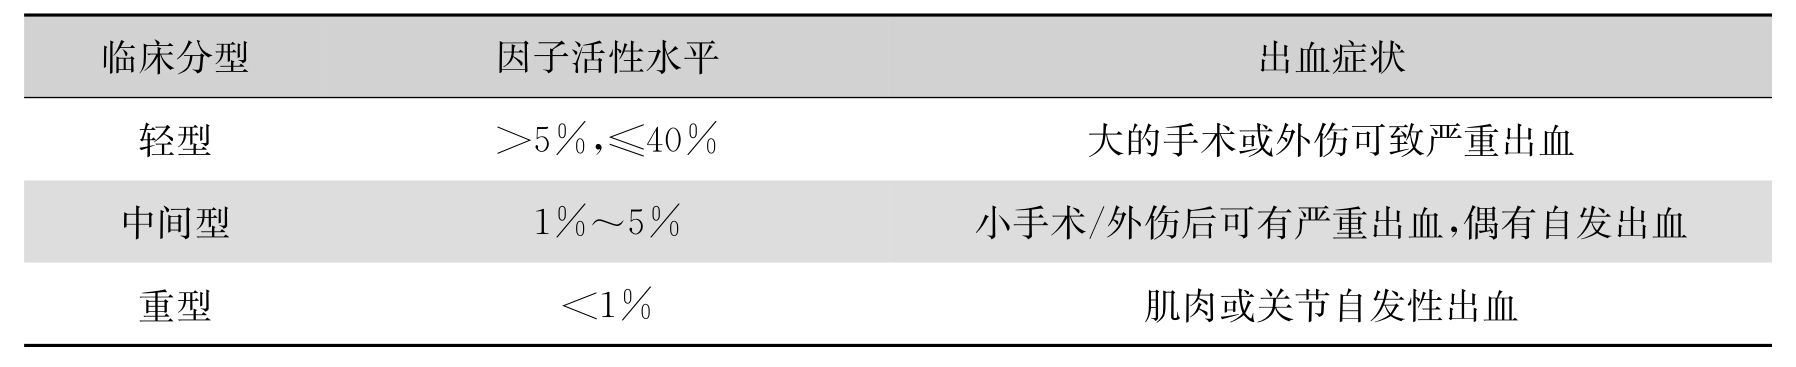
\includegraphics{./images/Image00204.jpg}
\end{minipage}}
\subfloat[心脏后前位X线图]{
\begin{minipage}[b]{0.48\textwidth}
\centering
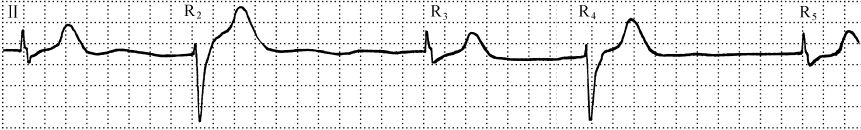
\includegraphics{./images/Image00205.jpg}
\end{minipage}}\\
\caption{}
\label{fig4-1-1}
\end{figure}

2.右前斜位 又称第一斜位,右胸前旋45°角。右前斜位最适合观察左心房、右心房体部,肺动脉主干和右心室漏斗部增大扩张。

心前缘分两段。上段由升主动脉构成,其下为肺动脉主干,右心室漏斗部(肺动脉圆锥)及右心室,近膈之一小段为左心室心尖部。两心室构成心前缘比率随旋转角度有所不同。左、右心室间无明显分界标志。

心前缘与胸壁之间有三角形透明区,尖向下,心位于胸骨与脊柱之间。心后缘分两段。上段由主动脉升部后缘、弓部、气管及上腔静脉重叠组成,除气管及其分叉部分外,难以区分。下段由心房构成,上部较长轻度向后凸出者为左心房,下部膈上一小段为右心房。后心膈角处有时可见一个斜三角形阴影,为下腔静脉投影。心后缘与脊柱之间较透亮的区域称为心后间隙。食管及降主动脉在心后间隙通过,食管中下段与左心房相邻,食管的移位是左心房增大的重要标志之一。

\begin{figure}
  \centering
\subfloat[心脏右前斜位线图]{
\begin{minipage}[b]{0.48\textwidth}
\centering
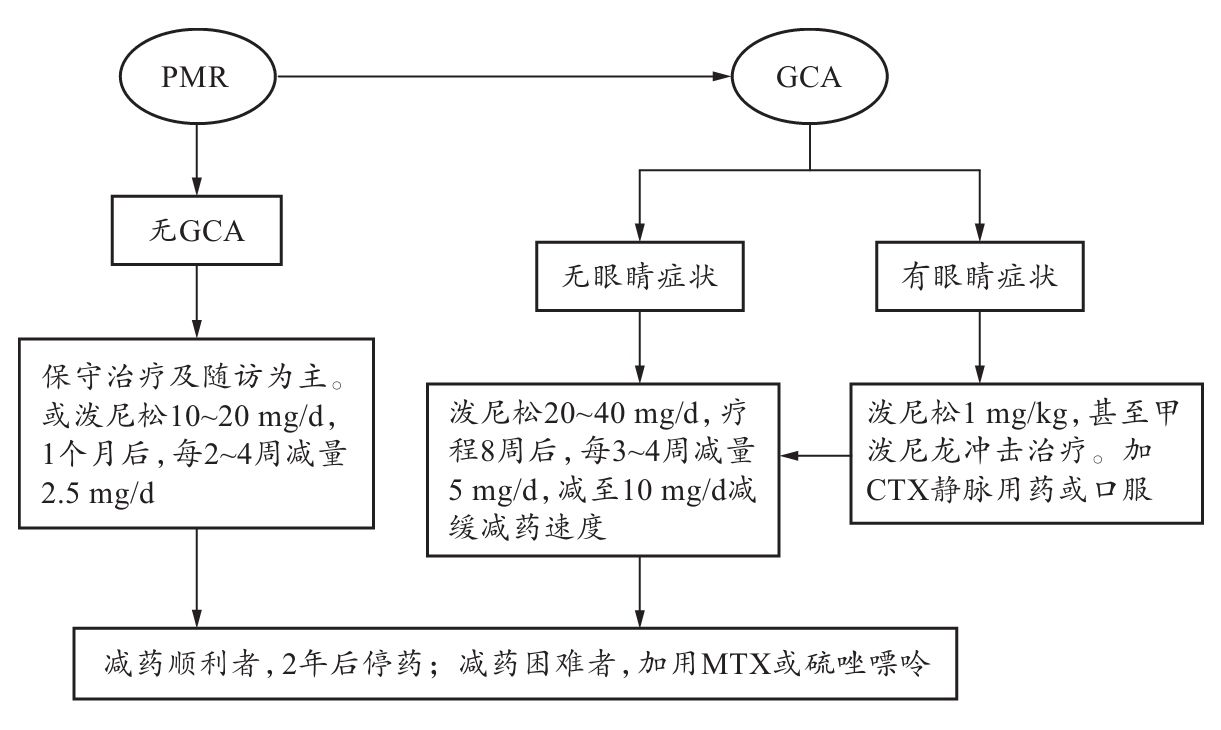
\includegraphics{./images/Image00206.jpg}
\end{minipage}}
\subfloat[心脏右前斜位食管吞钡X线图]{
\begin{minipage}[b]{0.48\textwidth}
\centering
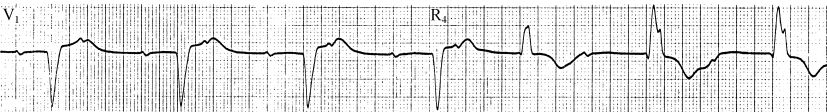
\includegraphics{./images/Image00207.jpg}
\end{minipage}}\\
\caption{}
\label{fig4-1-2}
\end{figure}

3.左前斜位 又称第二斜位或四腔心位,左胸前旋60°。室间隔与中心X线接近平行,故两心室大致是对称的,分为前后各半,前半为右心室,后半为左心室。两者几无重叠。左前斜位主要观察左、右心室,右心房和全部胸主动脉,对了解左肺动脉、左心房及其与左主支气管的关系,也有重要价值。

\begin{figure}
  \centering
\subfloat[心脏左前斜位线图]{
\begin{minipage}[b]{0.48\textwidth}
\centering
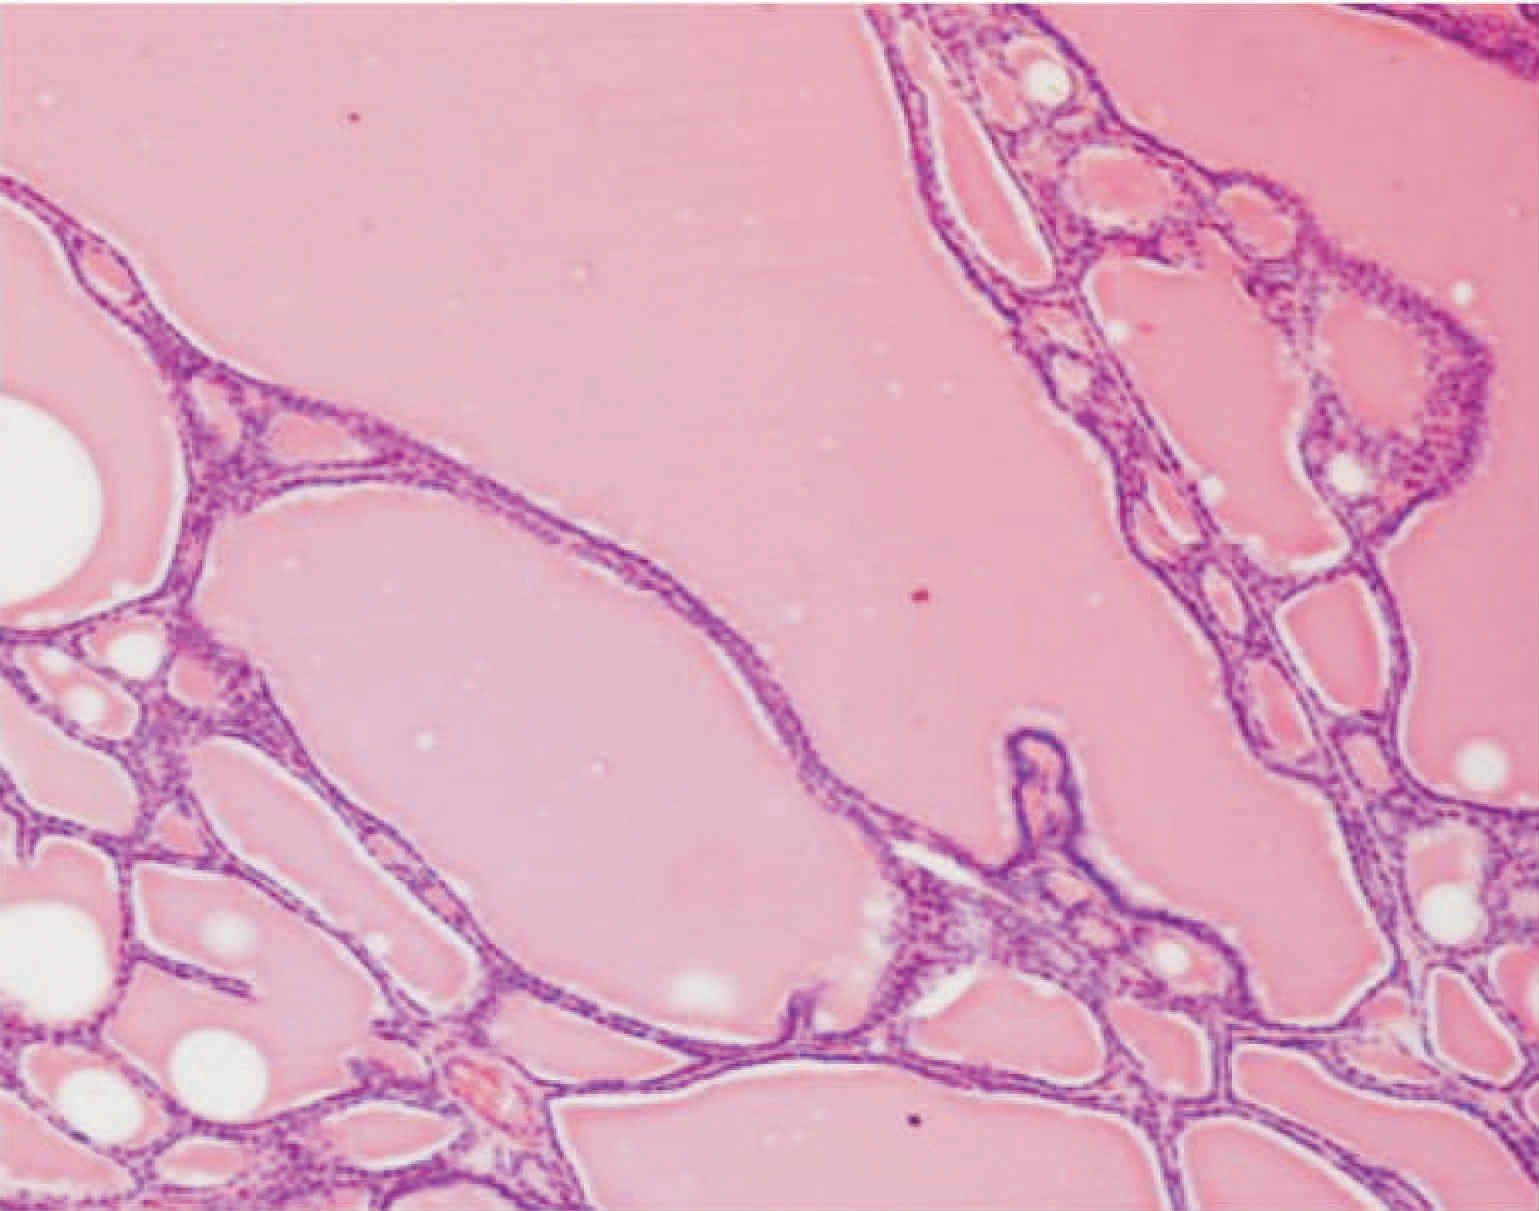
\includegraphics{./images/Image00208.jpg}
\end{minipage}}
\subfloat[心脏左前斜位X线图]{
\begin{minipage}[b]{0.48\textwidth}
\centering
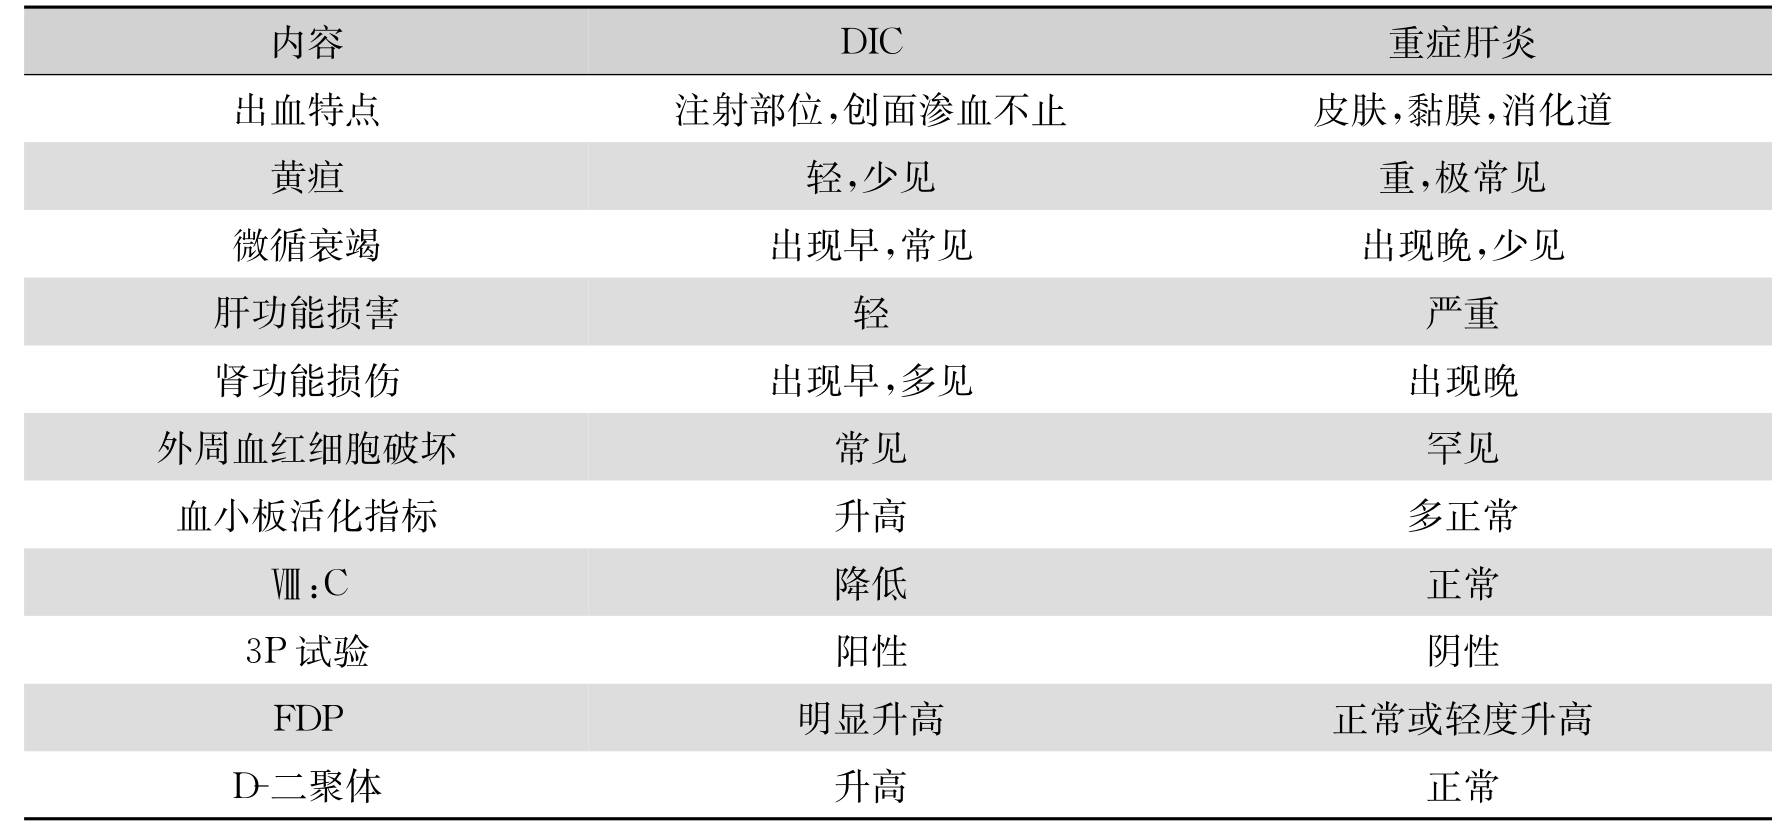
\includegraphics{./images/Image00209.jpg}
\end{minipage}}\\
\caption{}
\label{fig4-1-3}
\end{figure}

心前缘分为两段。上段为右心房、下段为右心室。右心房段主要由右心耳构成,房、室间界限不清。右心耳上方有一略凸向前的边缘,由升主动脉前缘构成,与右心耳之间有一浅切迹或近于垂直相连,主动脉前缘的上方与上腔静脉相重叠。心前缘与胸壁之间呈带状透明区,心、大血管影位于脊柱的右侧。

心后缘分两段。上段主要为血管结构,可见主动脉弓、弓下主肺动脉窗,窗内有气管、气管分叉、左右主支气管及与其伴行的左肺动脉和沿脊柱前缘下行的降主动脉的根部。下段为房、室阴影,其上部为左心房,下部为向后膨凸的左心室,有时两者间有一浅切迹为房室沟。深吸气时左室下可见一浅切迹,为室间沟,室间沟的位置是判断左、右心室增大的标志。后心膈角可见下腔静脉影。心后下缘、食管与膈之间的三角间隙为心后食管前间隙。

4.左侧位 心影由心尖到心底自前下向后上倾斜。左侧位主要观察左心,尤其是对左心房的观察较为满意。

心前缘分两段。下段为右心室前壁。上段由右心室漏斗部与肺动脉主干构成。上部心缘逐渐离开胸壁呈一浅弧向后上移行,其上方为升主动脉前壁,此等结构与胸骨后缘间形成的间隙称心前或胸骨后间隙,间隔下段为右心室沿胸壁向下与膈相重叠。

心后缘分两段。上段小部分为左心房,下段由左心室构成,轻度向后隆凸,后心膈角处可见三角形阴影为下腔静脉。

心脏膈面除前端一小部分为右心室外,主要由左心室构成。主动脉弓及主动脉窗因有部分重叠故均较左前斜位小。气管分叉前缘可见右肺动脉的轴位投影。

\begin{figure}
  \centering
\subfloat[心脏左侧位线图]{
\begin{minipage}[b]{0.48\textwidth}
\centering
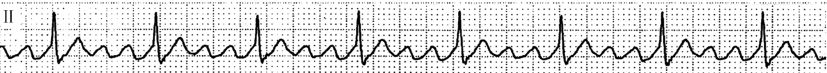
\includegraphics{./images/Image00210.jpg}
\end{minipage}}
\subfloat[心脏左侧位X线图]{
\begin{minipage}[b]{0.48\textwidth}
\centering
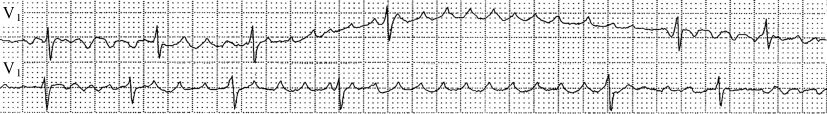
\includegraphics{./images/Image00211.jpg}
\end{minipage}}\\
\caption{}
\label{fig4-1-4}
\end{figure}

二、心脏测量

测量心脏大血管的目的是为了比较准确地估计大血管的大小、增大的程度以及治疗观察随访的对比依据。心脏大血管的测量方法很多,主要是常用的一些径线、心胸比率、心脏正面面积(心表面积)、心脏体积(容积)指数等。进行心脏大血管测量的标准正位片有规定的摄片条件,即:靶片距正位片2m、侧位片1.5m。在临床实践中使用最为广泛的是心胸比率法。

心胸比率法:心脏横径(\emph{T} \textsubscript{1} +\emph{T}
\textsubscript{2} )与胸廓横径(\emph{T}
)通过右膈顶的胸廓内径之比。男性平均为0.43±0.04,女性平均为0.44±0.03,临床上以0.5为正常上限,0.51~0.55为轻度,0.56~0.6为中等度,0.6以上为重度心脏增大。

\begin{figure}[!htbp]
 \centering
 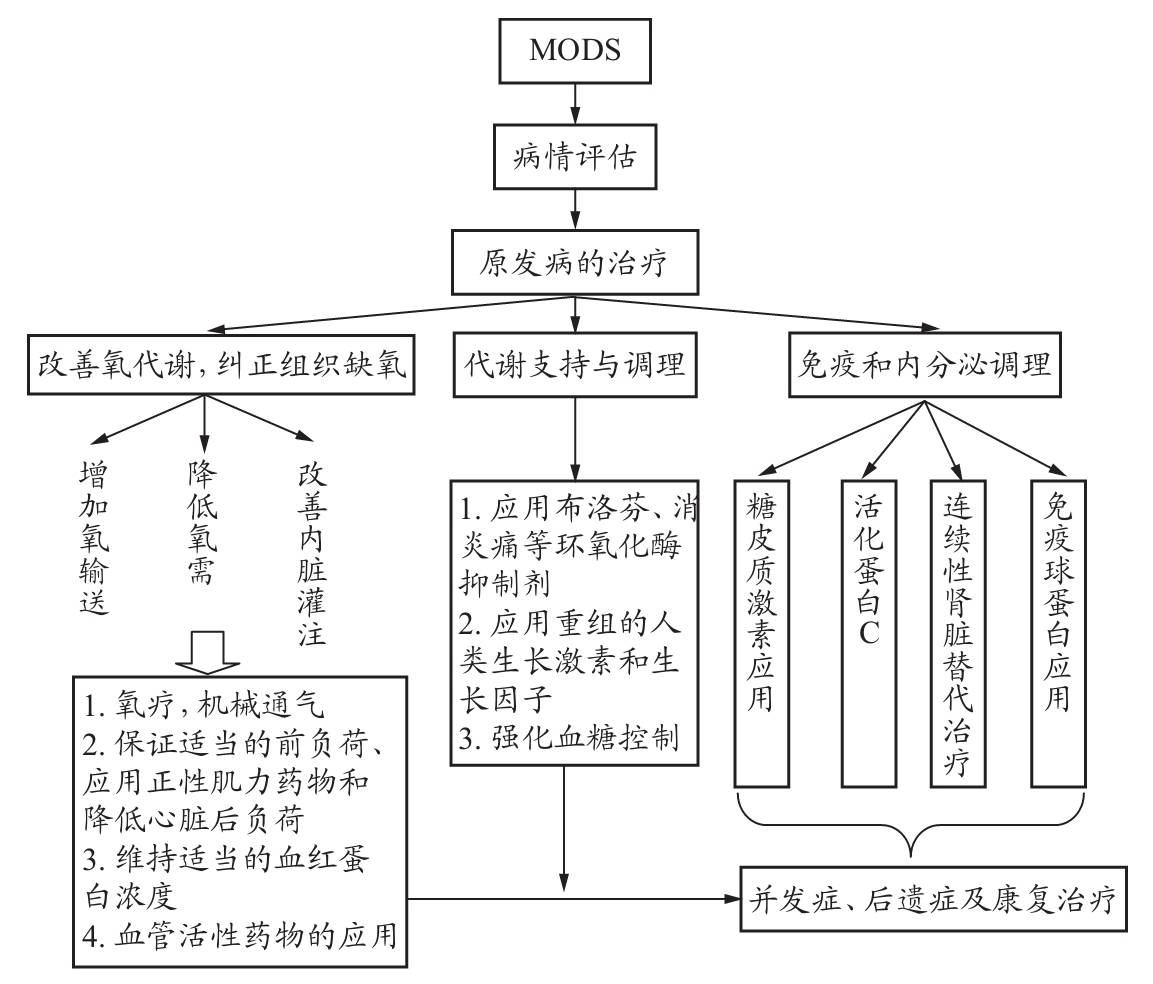
\includegraphics{./images/Image00212.jpg}
 \captionsetup{justification=centering}
 \caption{心脏横径、心胸比率测量示意图 {\small \emph{T} \textsubscript{1} 右心横径 \emph{T} \textsubscript{2}左心横径 \emph{T} \textsubscript{1} +\emph{T} \textsubscript{2}心脏宽径 \emph{T} 胸廓内径 \emph{OO} ′胸廓中线}}
 \label{fig4-1-5}
  \end{figure} 

\section{先天性心脏病}

\subsection{心房间隔缺损}

\begin{figure}[!htbp]
 \centering
 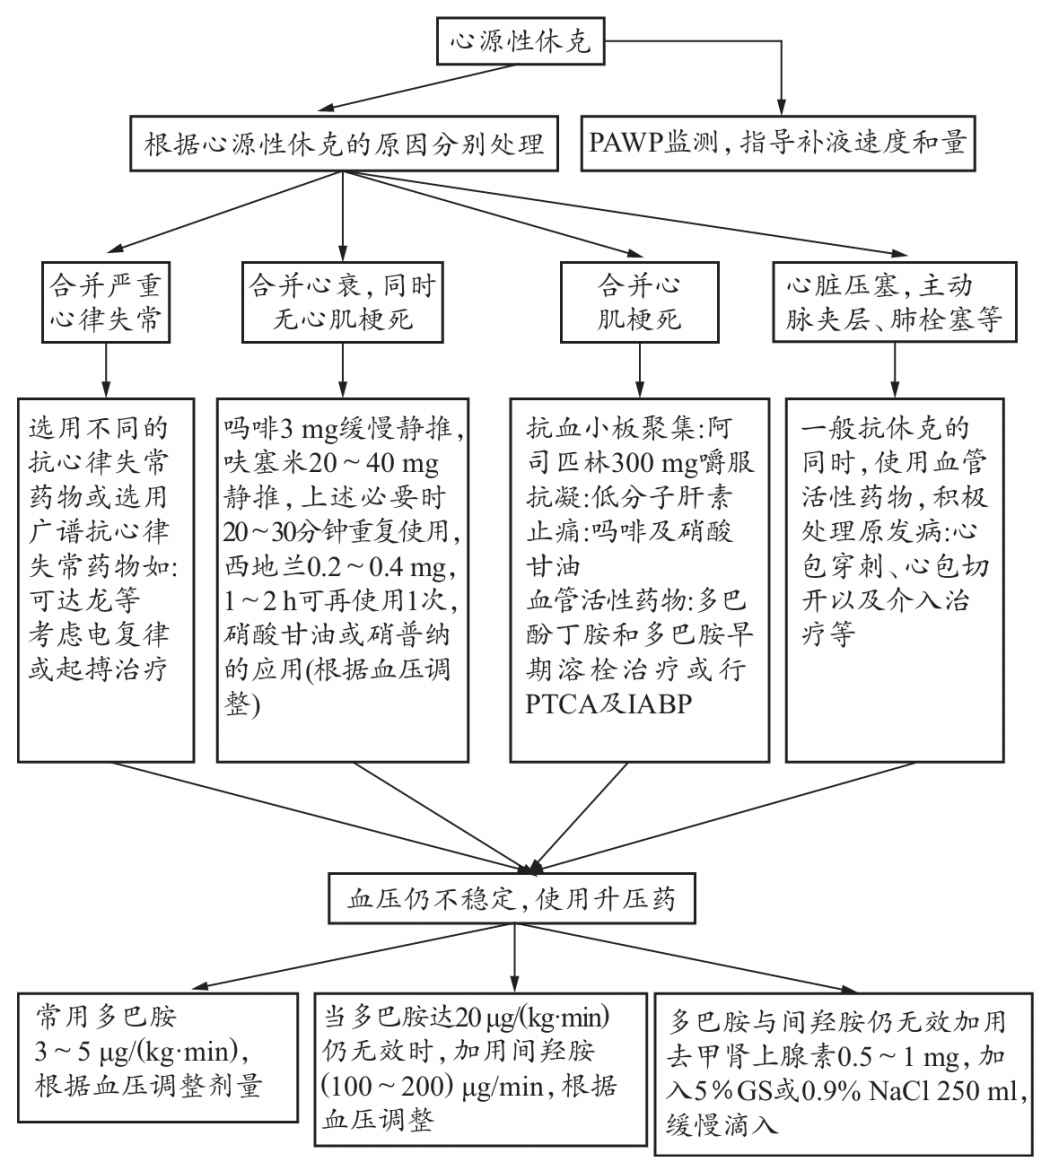
\includegraphics{./images/Image00213.jpg}
 \captionsetup{justification=centering}
 \caption{正位X线胸片示房间隔缺损}
 \label{fig4-2-1}
  \end{figure} 

\textbf{【病史摘要】}  男性,40岁。气急、胸闷伴喘息9个月,活动后加重。

\textbf{【X线表现】}
 心影呈梨形,主动脉结缩小,肺动脉段明显突出,右下肺动脉干增粗明显,右下心缘延长,向右稍突出,心尖圆钝上翘。两肺纹理增多,边缘锐利。左心房增大征象不明显。

\textbf{【X线诊断】}  先天性心脏病,房间隔缺损可能性大;肺动脉高压。

\textbf{【评  述】}
 房间隔缺损是先天性心脏病中最常见的一种病变。根据Abbott氏1000例尸体解剖中房间隔缺损居首位,占37.4%;在国内1085例先天性心血管疾病中,占21.4%,本病亦占首位。但因临床症状多不明显,常被忽视。本病男女之比为1∶2。

按胚胎发育可分为原发孔型、继发孔型和混合型。

1.原发孔型 根据其畸形程度不一,又可分为四类。

(1)单纯型:缺损的下缘为完整的心内膜垫,缺损的上缘为原发房间隔所形成的弧形边缘。

(2)部分房室通道:是原发孔中常见的一种病变,除单纯原发孔缺损外,二尖瓣的大瓣亦呈分裂状态,形成二尖瓣关闭不全,使左心室血液与左、右心房相互交通。

(3)完全房室通道:除上述部分房室通道病变外,兼有三尖瓣隔膜的分裂,使四个房室腔相互交通,称为完全房室通道。

(4)共同心房或称单心房腔:原发房间隔与继发房间隔均不发育,则形成共同心房。

2.继发孔型 主要是由于第二间隔的发育异常或第一间隔过度吸收,致第二间隔不能完全掩盖第一间隔上部的心房间孔所致。按缺损的部位可分为三个类型:

(1)中央型(卵圆孔缺损型):位于卵圆窝处,临床上最为常见。

(2)下腔型:缺损位于下腔静脉入口处,位置较低,下缘缺如,和下腔静脉入口没有明显分界。

(3)上腔型:位于卵圆孔上方,紧挨上腔静脉入口,上界缺如,常和上腔静脉相连。

3.混合型 以上两种类型混合存在。

正常左心房压力8~10mmHg,右心房压力4~5mmHg。心房间隔存在缺损时,左心房内血液可分流入右心房,分流量随两侧心房间的压力差和缺损大小而异。右心房同时接受自体循环回流来的静脉血和左心房分流来的动脉血,血容量明显增加,致使右心房、右心室和肺动脉血流量增加,从而加重右心的负担,右心房、右心室因负荷过大而发生肥厚、扩张,肺动脉发生充血。随着年龄的增长,肺血流持续增加,可导致肺小动脉管壁逐渐发生内膜增生和中层增厚,引起管腔狭小和阻力增加,继而出现肺动脉高压。由充血性(高流量)肺动脉高压发展到阻塞性肺动脉高压时,可导致双向或由右向左分流,此时临床上出现发绀,甚至右心衰竭。

房间隔缺损X线表现常见的征象有:右心房、右心室增大,肺充血。左心房、左心室血流量减少,可正常或萎缩,主动脉结缩小,肺动脉段多为中度以上的明显凸出。尤其是右心房增大为其主要的特征性改变,其表现在后前位上,心房段延长,向右凸出,右心房/心高比值>0.50。左前斜位,心前缘上段向前上膨凸,有些病例可有上、下腔静脉扩张,为右心房增大的间接征象。右心室增大,心影向左旋转,心尖圆钝而抬高。肺充血、肺门舞蹈、肺动脉高压表现。肺血增多,肺动脉扩张,外围分支增粗、增多,当晚期发生阻塞性肺动脉高压时,肺动脉段呈瘤样扩张,肺门动脉亦明显扩张,外围血管变细、稀疏。

本病体征不很明显的患者需与正常生理情况相鉴别:如仅在胸骨左缘第2肋间闻及2级吹风样收缩期杂音,伴有第二心音分裂或亢进,则在正常儿童中亦常见到,此时如进行X线、心电图、超声心动图检查发现有本病的征象,才可考虑进一步做右心导管检查等确诊。

与较大的心室间隔缺损相鉴别:因左至右的分流量大,其X线、心电图表现与本病可极为相似,体征方面亦可有肺动脉瓣区第二心音的亢进或分裂,因此可能造成鉴别诊断上的困难。但室间隔缺损杂音的位置较低,常在胸骨左缘第3、4肋间,且多伴震颤,左心室常有增大等可资鉴别。但在儿童患者,尤其是与第一孔未闭型的鉴别仍然不易,此时超声心动图、右心导管检查等有助于确立诊断。此外,左心室右心房沟通(一种特殊类型的心室间隔缺损)的患者,其体征类似高位心室间隔缺损,右心导管检查结果类似心房间隔缺损,也要注意鉴别。

与瓣膜型单纯肺动脉口狭窄相鉴别:其体征、X线和心电图的表现,与本病有许多相似之处,有时可造成鉴别上的困难。但瓣膜型肺动脉口狭窄时,杂音较响,常伴有震颤,而肺动脉瓣区第二心音减轻或听不见;X线片示肺野清晰,肺纹稀少,可资鉴别。超声心动图见肺动脉瓣的异常,右心导管检查发现右心室与肺动脉间有收缩期压力阶差,而无分流的证据,则可确诊。

与原发性肺动脉高压相鉴别:其体征和心电图表现,与本病颇为相似;X线检查亦可发现肺动脉主干弧形凸出,肺门血管影增粗,右心室和右心房增大;但肺野不充血或反而清晰,可资鉴别。右心导管检查可发现肺动脉压明显增高而无左至右分流的证据。

多数房间隔缺损X线表现典型,诊断不难,且可粗略估计左向右分流量及肺动脉高压程度。小房间隔缺损X线改变轻或为正常范围,诊断要结合临床体征;二维超声心动图及彩色Doppler有助于确定诊断。房间隔缺损合并重度肺动脉高压,右心房室高度增大,杂音可不典型,有或无发绀,常需与其他水平分流的先天性心脏病相鉴别,超声心动图及心血管造影检查有重要意义。MRI因设备昂贵,仅用于疑难病例而又不适于做心血管造影者。对不典型病例,在临床上极易与肺动脉瓣狭窄、小的室间隔缺损及特发性肺功脉扩张相混淆,需做心导管检查确诊。

\subsection{心脏室间隔缺损}

\begin{figure}
  \centering
\subfloat[室间隔缺损术前]{
\begin{minipage}[b]{0.48\textwidth}
\centering
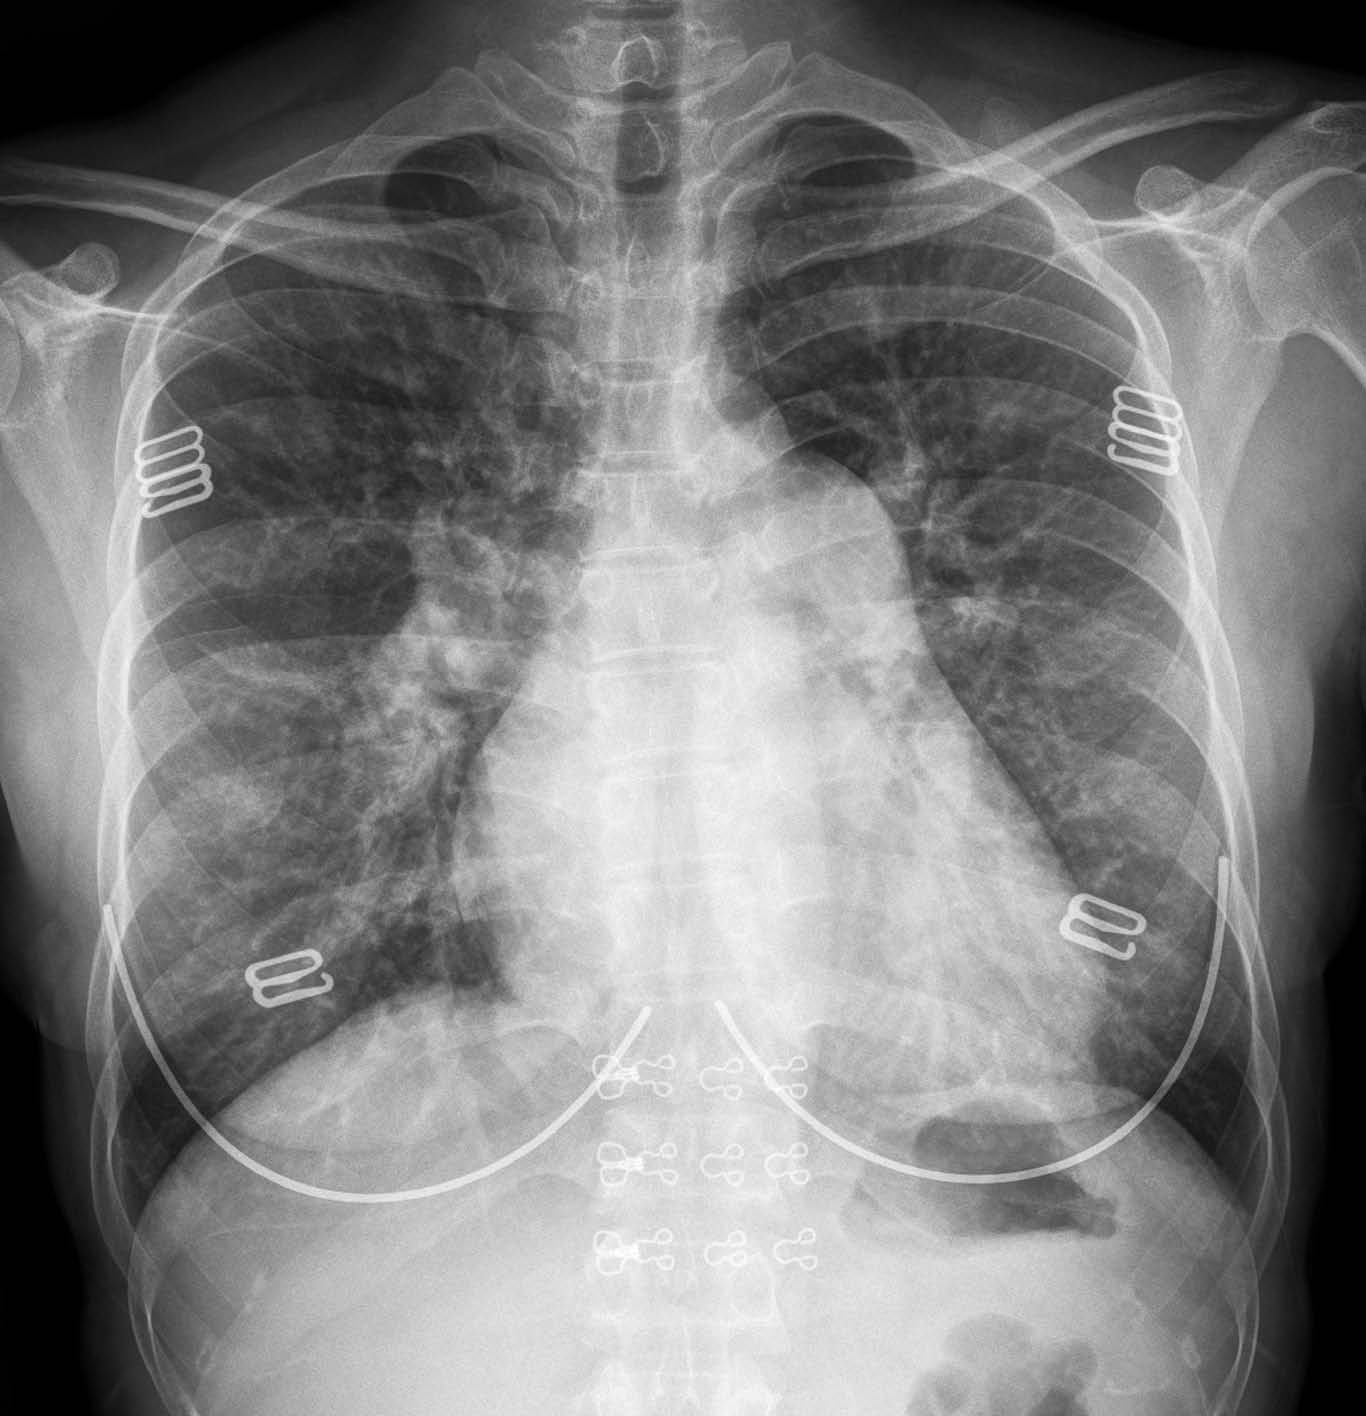
\includegraphics{./images/Image00214.jpg}
\end{minipage}}
\subfloat[室间隔缺损术后]{
\begin{minipage}[b]{0.48\textwidth}
\centering
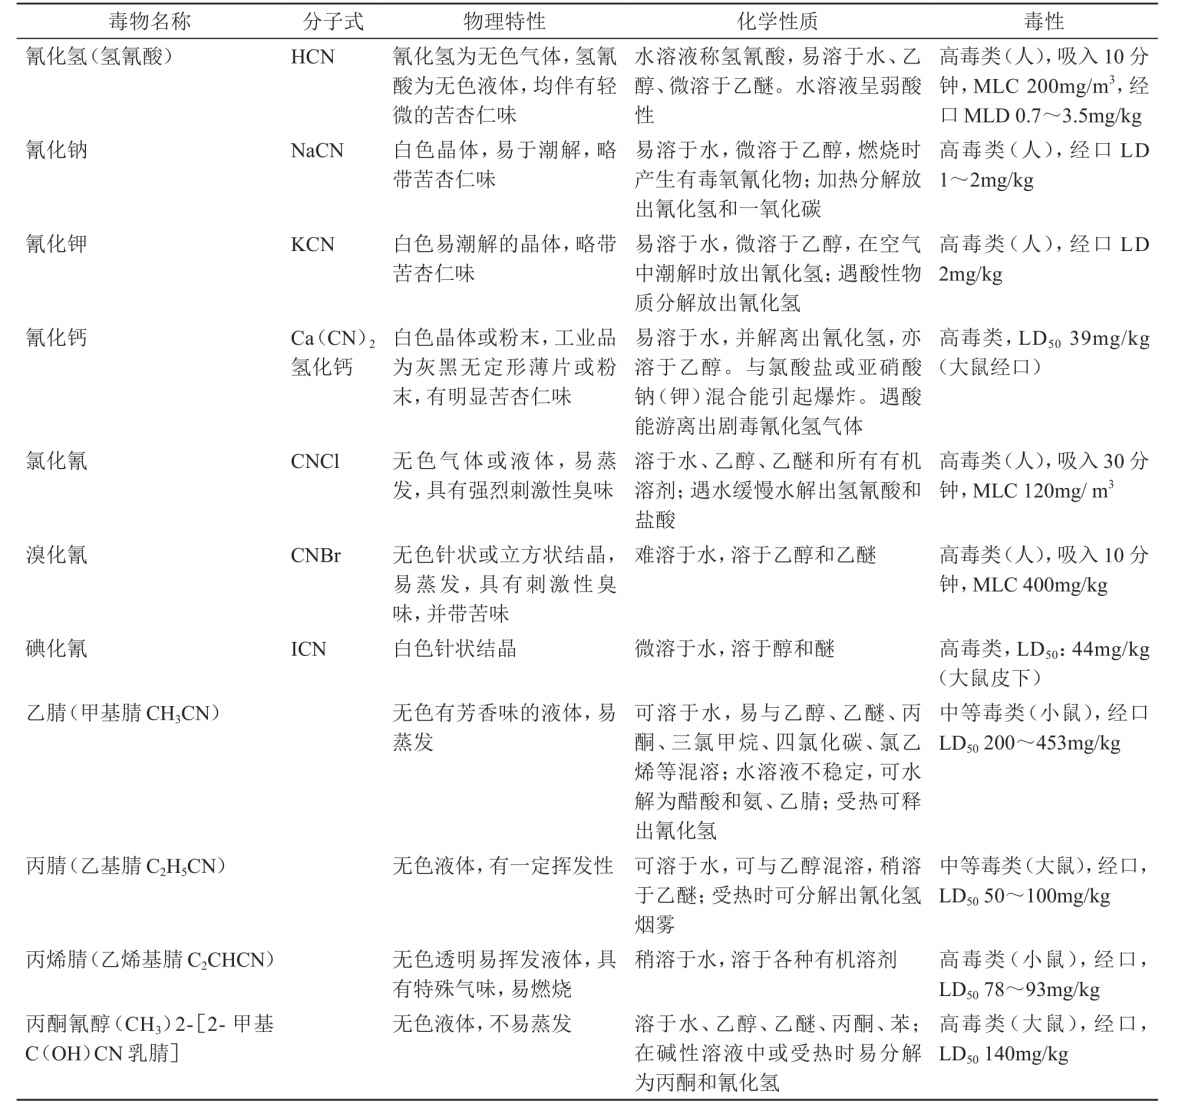
\includegraphics{./images/Image00215.jpg}
\end{minipage}}\\
\caption{}
\label{fig4-2-2}
\end{figure}

\textbf{【病史摘要】}
 女性,38岁。体检时发现心脏杂音1年余。体格检查:胸骨左缘3、4肋间隙可扪及收缩期细震颤,并可听到Ⅲ、Ⅳ级收缩期杂音,肺动脉瓣区第2心音亢进。

\textbf{【X线表现】}
 心影呈梨形,主动脉缩小,肺动脉明显突出,右下肺动脉干增粗,左心缘向左扩大,心尖左下移位。两肺纹理增多,边缘锐利,呈肺充血改变。术后示两肺充血、肺动脉高压征象改善,心影缩小。

\textbf{【X线诊断】}  先天性心脏病:室间隔缺损(术前、术后)。

\textbf{【评  述】}
 本病是常见的先天性心脏病之一。国内1085例先天性心脏病的统计,本病发病率为15.5%,占第三位,在Abbott氏1000例尸检中,占5.5%,男性较多见。一般所称的心室间隔缺损系指单纯的缺损而言。它也可作为复杂的先天性畸形中的一部分而存在,如法洛四联症。

1.根据缺损大小及分流量分类

(1)小型缺损伴小分流量,缺损直径不超过0.5cm,无临床症状,左向右分流量很小,一般称之为Roger氏病。

(2)中等大小的缺损伴大分流量,缺损直径在0.5~1.5cm,左向右分流量较大,右心室及肺动脉压力有一定程度增高。

(3)大型缺损伴左向右分流,缺损直径大于1.5cm,肺动脉阻力增高,有时左、右心室压力可以相接近。

(4)大型缺损伴右向左分流,大型缺损到后期肺血管阻力超过体循环阻力,心室水平产生右向左分流。临床出现青紫。此类型称为艾森曼格氏综合征。

本病缺损多为单发,呈圆形或椭圆形,直径在5~35mm之间,以10mm左右大小为最常见。

2.根据缺损解剖部位分类

(1)嵴上型缺损位置较高,位于室上嵴前上方和主肺动脉瓣下,占室间隔缺损的15.6%。

(2)嵴下型缺损为膜部间隔缺损,位于室上嵴的后下方,此型缺损较大,发病率最高,占室间隔缺损的60.2%。

(3)隔瓣后缺损位于三尖瓣隔膜的后方,较前二型更居后,占室间隔缺损的21.3%。

(4)肌部缺损最少见,缺损可位于肌部间隔的任何部位,多数缺损靠近心尖,一般缺损较小,所谓罗格氏病(Roger氏病)多属此型,占室间隔缺损的2.9%。

心室的变化主要决定于缺损的大小和分流量,与两心室压力差别有关。正常时,左心室压力高于右心室压力。因此,左心室的血通过缺损流入右心室,产生自左向右分流,临床上无发绀现象。缺损大者,大量的分流血液自左心室流入右心室及肺动脉内,以致右心室及肺动脉内血液大增,肺动脉的流量可达体循环的3~5倍,从而产生肺充血、肺动脉高压、肺小动脉继发性病变以及两心室增大。最后由于肺循环的高压和肺小动脉阻力增高,右心室内压力超过左心室,则产生血液自右向左分流,临床上产生青紫。

室间隔缺损的心肺X线改变常取决于缺损的大小、心内分流和肺动脉高压三者的相互关系。小的缺损病例心肺X线所见于正常范围。典型者左、右心室明显增大,以左心室为著。肺多血改变,肺动脉段突出,肺门动脉扩张且搏动增强。

1.缺损较小,左向右分流量甚少,心脏形态和大小没有明显改变 有时仅表现为肺动脉段轻度凸出,肺纹理略增粗、增多,少数可有心脏轻度增大。主动脉结多属正常。X线表现甚难与正常者区别。诊断要靠临床体征。

2.缺损较大,左向右分流量较多,可出现明显的X线改变 心脏外形呈“二尖瓣”型。心脏呈中-高度增大,左、右心室均增大,但多数病例仍以右心室增大显著。由于血流量增加,左心房也常轻度增大。肺动脉段呈中-高度凸出,肺门动脉扩张,搏动增强,肺血增多。主动脉结正常或轻度缩小。

3.室间隔缺损伴有明显肺动脉高压 右心室压力接近或超过体循环水平时,发生右向左分流。临床上出现发绀,即所谓艾森曼格氏综合征。心脏和左、右心室增大更为明显。在肺血增多的基础上,肺动脉高压征象更明显。肺动脉段高度凸出,部分病例瘤样扩张,肺门血管也相应地明显扩张,外围分支细少,呈残根状,肺野变清晰。

在先天性心脏病中动脉导管未闭虽有左心室增大,但右心室无增大,主动脉结亦增大,可与本病相鉴别。

与房间隔缺损鉴别可有以下特点:①室间隔缺损不引起右心房的增大。②左心室及主动脉球无萎缩变小。③肺门充血程度较轻。④心前区杂音位置较低。

多数室间隔缺损X线表现典型诊断不难且可粗略估计左向右分流量的大小及肺动脉高压的程度;小室间隔缺损X线改变轻微或在正常范围内,诊断主要靠典型的临床体征和Doppler超声心动图检查;室间隔缺损合并重度肺动脉高压,右心房室增大明显,杂音可不典型,有或无发绀,常与其他左向右分流或双向分流畸形伴有肺动脉高压者混淆,需借助超声心动图甚至造影检查做出鉴别。

\subsection{动脉导管未闭}

\begin{figure}[!htbp]
 \centering
 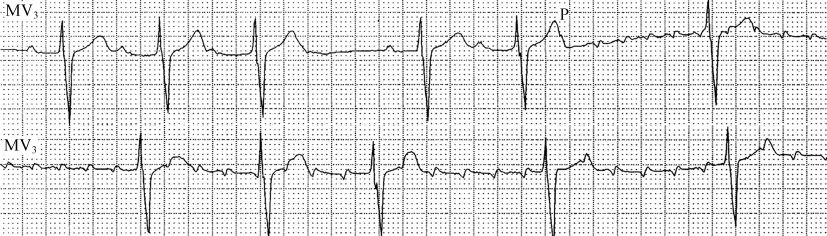
\includegraphics{./images/Image00216.jpg}
 \captionsetup{justification=centering}
 \caption{正位X线胸片,动脉导管未闭}
 \label{fig4-2-3}
  \end{figure} 

\textbf{【病史摘要】}
 女性,8岁。体检时发现心脏杂音3天。体格检查:一般情况可,胸骨左缘第2、3肋间听到响亮的连续性机器样杂音,有轻微震颤,肺动脉瓣区第2心音亢进。

\textbf{【X线表现】}
 心影呈梨形,主动脉结无明显缩小,肺动脉段突出,主动脉在动脉导管附着处呈局部漏斗状扩张,即漏斗征。右肺门血管影增多、浓密,右心缘见双房影,心尖左下移位。两肺纹理增多,边缘锐利,呈肺充血改变。支气管分叉角增大,大于90°。

\textbf{【X线诊断】}  先天性动脉导管未闭。

\textbf{【评  述】}
 本病是常见的先天性心脏病之一,国内资料1085例先天性心脏血管病的统计,发生率占21.1%,居第二位,女高于男,为3~5∶1。

病理分类:

1.圆柱型 导管两头粗细一致,状如圆柱,也称管状型。

2.漏斗型 导管于主动脉端粗,肺动脉端细,形如漏斗。

3.缺损型(窗型) 导管极短,没有长度,主动脉与肺动脉紧贴,形成缺损孔道。

4.动脉瘤型 导管呈瘤样扩大。

随动脉导管的粗细病变严重的程度不同而临床表现、X线表现也不同。导管细,分流量小,可无症状;导管粗,分流量大,可影响发育、乏力、心悸、气喘,如肺动脉高压;产生右向左分流,则半身出现发绀;晚期可出现心力衰竭。听诊,胸骨左缘第2肋间有连续性机器样杂音,并可触及震颤。

常见X线表现有:①心脏大小和外形:心脏大小的变化与导管的粗细、分流量的大小有关。导管粗,分流量大,心脏增大可很明显;导管细,分流量小,心脏亦可不扩大或轻度增大。心影外形呈二尖瓣型或二尖瓣-主动脉型。②肺血管的表现:肺充血,肺动脉分支扩张、增粗和迂曲,但血管轮廓清晰。肺充血的程度与导管粗细、分流量的大小成正比。一般充血者比较明显,引起充血性肺动脉高压。少数病例见到肺门舞蹈,但不如房间隔缺损多见。晚期可导致梗阻性肺动脉高压。③左心房增大:由于血流量增多,左心房可发生扩大,程度一般较轻。④左心室增大:主要表现在流出道,左心室扩大的程度与分流量也成正比。⑤升主动脉及主动脉结增宽,搏动明显增强:一般认为,凡是左向右的心内分流,主动脉影不增宽或缩小,尤以房间隔缺损缩小比较明显。如为心外分流,则见主动脉增宽,搏动增强。⑥肺动脉段突出:呈轻度至中度突出,明显突出的较为少见。⑦右心室增大:一般早期右心室不增大,如伴有肺动脉高压,右心室可增大。⑧漏斗征:是指主动脉在动脉导管附着处呈局部漏斗状扩张。表现为主动脉弓阴影下方并不随即内收而继续向左外膨隆,并逐渐过渡至降主动脉,随后再向内呈斜坡状移行于降主动脉阴影。⑨动脉导管瘤:多表现为左上纵隔的搏动性肿块。侧位在主动脉弓下、降部前方、主动脉窗内。

主动脉结增宽和漏斗征、左心室及主动脉搏动增强等征象三者间并无大差别,这对本症与其他左向右分流引起肺动脉高压的鉴别诊断是有帮助的。漏斗征的病理基础是动脉导管起始部主动脉管腔的漏斗状扩张。

与主动脉窦瘤破裂的鉴别在于其患者既往无心脏病的症状和体征,而在成年后突然发病,且迅速出现心力衰竭和心影增大,左右心腔均受累,以左心室增大为主,心影近似主动脉型。动脉导管未闭无右心室增大,不会在短期内出现心影增大和心力衰竭的征象,且自幼即有心脏病的相应症状和体征。

粗大的动脉导管未闭其临床表现和普通X线检查,几乎难与主动脉-肺动脉间隔缺损鉴别,后者由于缺损的位置特点,一般杂音位置较低。胸主动脉造影为最重要的诊断和鉴别诊断方法。

\subsection{肺动脉瓣狭窄}

\begin{figure}[!htbp]
 \centering
 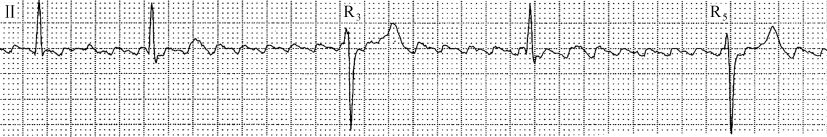
\includegraphics{./images/Image00217.jpg}
 \captionsetup{justification=centering}
 \caption{正位X线胸片,肺动脉瓣狭窄}
 \label{fig4-2-4}
  \end{figure} 

\textbf{【病史摘要】}
 男性,23岁。劳累后心悸、气急3年,常觉无力。体格检查:胸骨左缘第2肋间闻及响亮、粗糙的收缩期杂音,伴有震颤,肺动脉瓣区第2心音减低,可听到肺动脉区喷射音。

\textbf{【X线表现】}
 心脏呈二尖瓣型,心影轻度增大,以右心室增大为主,主动脉结缩小,肺动脉段瘤样突出,心尖圆钝上翘。两肺纹理纤细、稀疏,两肺野透亮度增加,呈少血改变。两肺门动脉阴影不对称(左侧>右侧)。

\textbf{【X线诊断】}  先天性肺动脉瓣狭窄。

\textbf{【评  述】}
 临床及X线表现随狭窄的程度而不同,常见症状易疲乏,劳累后心悸、气急,一般症状较轻。严重狭窄易导致卵圆孔的开放。可出现发绀,体检胸骨左缘第2前肋间听到3~4级收缩期杂音,伴有震颤,肺动脉瓣区第2心音减弱或消失。心电图电轴右偏,右心室肥厚,右束支传导阻滞,右心房肥大。

1.按其狭窄部位和病理改变可以分为以下四个类型:

(1)瓣膜狭窄:最为常见,占70%~80%,瓣膜缘不同程度的粘连愈着,形成向肺动脉干腔内呈圆顶样突出的隔膜,于中心或偏心有一狭窄瓣孔,其大小从几毫米至10mm以上,伴有肺动脉主干的狭窄后扩张。瓣膜呈不同程度的增厚,甚至变形。

(2)漏斗部狭窄(瓣下狭窄):较少见,约占10%,狭窄可位于右心室流出道的任何部位,可为狭长的肌肉型通道管样狭窄,亦可为环状狭窄的隔膜型。

(3)瓣上狭窄:于肺动脉瓣上,即肺动脉干根部局限性狭窄。

(4)混合型狭窄:如肺动脉瓣狭窄合并漏斗部狭窄,或肺动脉瓣狭窄合并轻度瓣上狭窄。

2.病理生理

(1)肺动脉瓣膜部狭窄X线表现:①心脏呈二尖瓣型,心脏大小正常或轻度增大者居多。少数为中度至高度增大,主要为右心室增大,正位显示心尖圆钝且向上翘,约有1/3病例可见右心房增大,显著增大者常提示重度肺动脉瓣狭窄或合并三尖瓣关闭不全。②肺动脉段凸出为狭窄后扩张所致,多呈直立式,其上缘可接近主动脉弓水平,凸出的肺动脉段多为中度至高度凸出,与左心缘连接处凹陷。③肺血减少,肺血管纹理纤细、稀疏,尤其与肺动脉段明显凸出形成鲜明对比,为肺动脉瓣狭窄常见的征象,且多反映为较重的狭窄。右肺门动脉因距离肺动脉主干较远影响较小,肺纹理多细小。左肺门动脉亦见扩张,大于右侧致使两肺门阴影不对称,左侧>右侧。在诊断上具有重大意义。④心脏大血管搏动,心缘搏动正常或增强。肺动脉段及左肺门搏动增强,右肺门动脉无搏动而呈静止状态,两者形成鲜明对比,对诊断具有较大意义。

(2)肺动脉瓣漏斗部狭窄X线表现:漏斗部肌性狭窄,肺动脉段凹陷,心尖上翘,心脏呈靴形,心外形似四联症,另有少数病例肺动脉段轻度膨凸,心外形似二尖瓣型,右心室多呈不同程度增大,于肺动脉段下方常可见轻度膨凸,为漏斗部心腔,第三心室的反映。肺血减少表现。

(3)肺动脉瓣上狭窄及混合型狭窄:较少见,其X线表现有上述相应的征象。

肺动脉狭窄基本的血流动力学变化是右心排血受阻。右心室收缩压升高而肺动脉压正常或降低,结果产生右心室肥厚,以至于继发右心衰竭。肺动脉瓣狭窄,因血流动力学影响,即血液冲击狭窄瓣口后产生的涡流引起肺动脉主干的扩张,称为狭窄后的扩张,可波及左肺动脉为瓣膜狭窄的特征之一。

先天性肺动脉狭窄为常见的先天性心脏病,普通X线检查多可以做出定性诊断,但在病变程度的估计上,尤其心脏不大或仅轻度增大者,常有一定限度。单发的漏斗部狭窄较少见,平片诊断受到一定限制,常需注意与无发绀的四联症相鉴别。二维超声心动图及彩色Doppler有助于确定诊断。右心导管检查可作为诊断及狭窄程度判断的重要依据。为了进一步明确瓣膜、漏斗部狭窄以及右心室肥厚的解剖诊断和形态特点,以助于疑难病例鉴别诊断和手术治疗适应证的选择,右心室造影在临床上具有重要意义。

\subsection{法洛四联症}

\begin{figure}[!htbp]
 \centering
 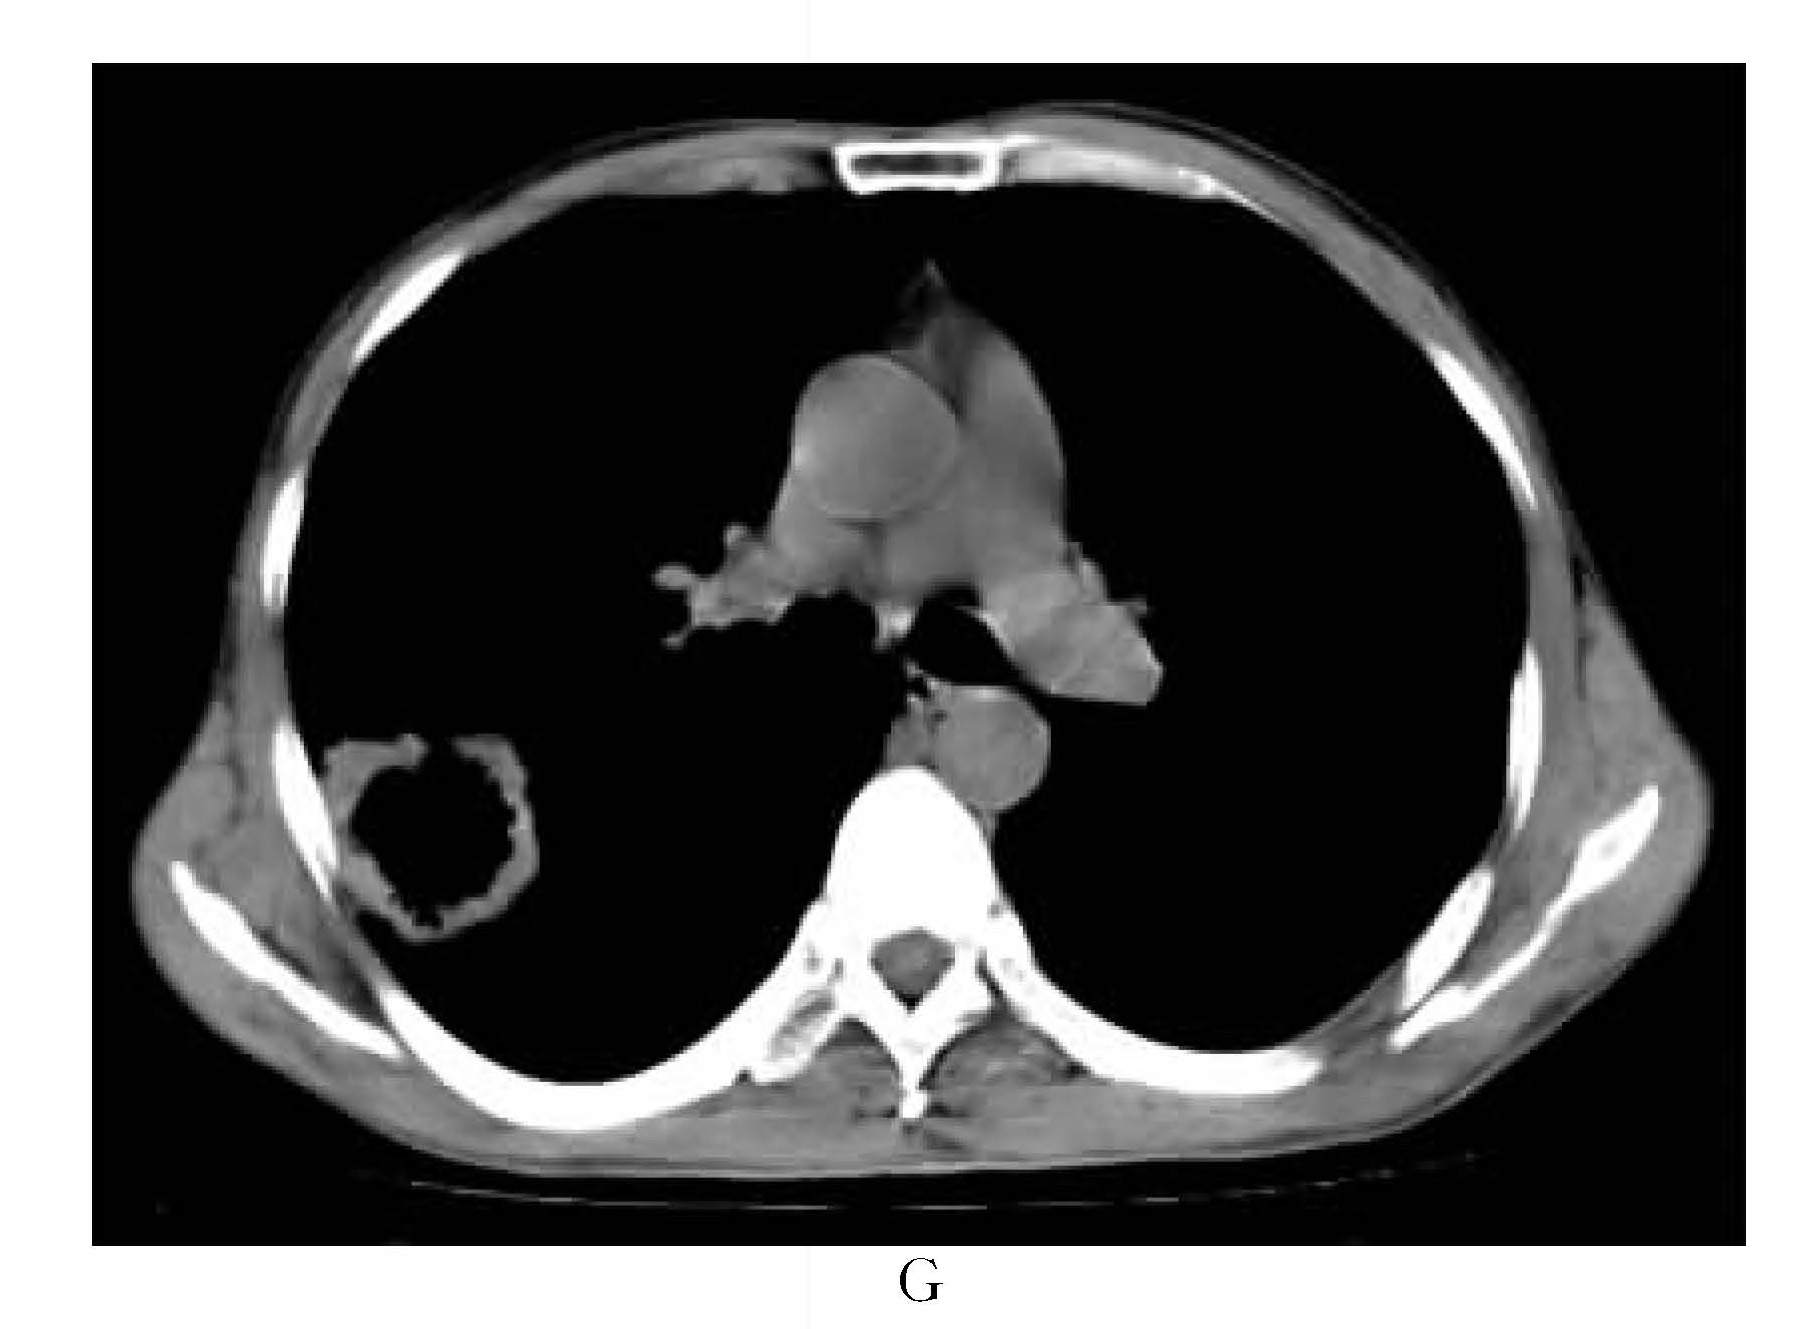
\includegraphics{./images/Image00218.jpg}
 \captionsetup{justification=centering}
 \caption{正位X线胸片,法洛四联症}
 \label{fig4-2-5}
  \end{figure} 

\textbf{【病史摘要】}
 男性,21岁。活动后气促、呼吸困难10多年,平时喜欢蹲踞。患者发育迟缓,体格弱小,嘴唇发绀,胸骨左缘2、3肋间有Ⅱ~Ⅲ级收缩期喷射性杂音,心电图检查提示右心室肥厚。

\textbf{【X线表现】}
 心影略呈靴型,心腰凹陷,心尖上翘,示右心室增大。肺血减少,肺内血管纹理稀疏、纤细,肺门阴影小。

\textbf{【X线诊断】}  先天性心脏病:法洛四联症。

\textbf{【评  述】}
 患儿通常在1岁左右出现发绀,在哭闹时或活动后加重,喜蹲踞。缺氧发作时可出现晕厥、呼吸困难、意识丧失、抽搐等。患者有发育迟缓,消瘦,杵状指、趾,胸骨左缘2~4肋间可闻及收缩期3级以上杂音,P2减弱或消失、红细胞增加。心电图有心室肥厚伴劳损,右心房肥大,不完全性右束支传导阻滞。

1888年由法国人Fallot氏首先描述了肺动脉狭窄(常为右心室漏斗部狭窄)、室间隔缺损、主动脉骑跨、右心室肥厚,即法洛四联症。占先天性心脏病的9.2%~14%,在先天性发绀型心脏病中占第一位,为66%~75%。约1/4病例可伴有房间隔缺损,即法洛五联症。四联症主要畸形为肺动脉狭窄和高位室间隔缺损。

肺动脉狭窄的程度可由轻度狭窄到完全闭锁,狭窄的部位多为漏斗部狭窄,或兼有肺动脉瓣的狭窄。漏斗部狭窄可以为整个漏斗部的狭窄,也可为局限性环形狭窄。后者可造成狭窄与瓣膜之间的扩张,形成所谓第三心室。室间隔缺损是高位的,多为膜部缺损,缺损直径往往在1cm以上。主动脉骑跨程度不等,升主动脉都较粗大,20%~30%患者合并右位主动脉弓。右心室肥大是一种代偿性肥厚,其室壁厚度可达左心室,甚至超过左心室,左心室则发育不良。

四联症的血流动力学改变主要取决于肺动脉狭窄所形成的阻力,狭窄愈重,右心室排血阻力愈大,通过室间隔缺损由右向左的分流量也就愈大。主动脉同时接受来自左、右心室的混合血,使体循环血氧饱和度降低,而肺动脉血流量减少进一步加剧缺氧,从而引起发绀。部分病例肺动脉狭窄较轻,室间隔缺损也很少,右心室压力常低于左心室或相仿,不出现由右向左分流或无发绀。此外,发绀型四联症几乎都有来自体循环的侧支血管供应肺循环,侧支循环一般占主动脉血流量的5%~30%,丰富的侧支循环可以改善缺氧从而减轻发绀。

典型四联症的X线表现:①心脏呈木靴状,右心室肥厚增大,将左心室推向后上方,以致心尖圆钝而翘起,心腰凹陷及主动脉升部、弓部扩张。某些病例肺动脉段下方略见膨凸,系第三心室所致。少数病例可见右心房增大和上腔静脉扩张,左心房、左心室都不见增大。②肺血减少,肺门阴影缩小,肺内血管纹理细小、稀疏。某些病例肺门阴影显著缩小或无明显的动脉支干阴影。而肺门区出现粗乱的血管阴影或肺野血管纹理呈网状时,为侧支循环的表现。二者均为肺动脉狭窄较重的指征。③主动脉升、弓部扩张增宽,有1/4~1/3合并右位主动脉弓。

重症四联症的X线表现:心脏外形与典型四联症的心脏形态基本相似,仅是增大程度上的区别。重型病例心脏增大较明显,心腰凹陷和主动脉升弓部扩张增宽更加显著,多数病例示侧支循环表现。

轻度可无发绀型四联症的X线表现:心脏外形和肺血减少的X线表现取决于肺动脉狭窄和室间隔缺损的程度,不一定都具有上述典型的X线征象。如室间隔缺损较小,肺动脉狭窄亦轻,则心脏形态的改变与单纯肺动脉狭窄相仿。如室间隔缺损较显著,而肺动脉狭窄不显著,则心脏形态的改变与室间隔缺损相仿。

根据X线的典型征象结合临床体征(尤其是发绀),X线平片多能做出或提示四联症的诊断,年龄越大越可靠;在婴幼儿相同的X线征象常与其他肺血少伴发绀的复杂心脏畸形相混淆,如四联症伴有肺动脉狭窄的右心室双出口、大动脉错位、单心室、三尖瓣闭锁、肺动脉闭锁及右心发育不全等,X线平片诊断受到限制。X线征象拟似四联症,但心脏明显增大、心脏异位或疑有左位升主动脉者,特别是心电图无右心室肥厚时应警惕其他复杂畸形。超声心动图在四联症无创性检查中有重要作用,可部分取代造影检查。对上述疑难病例和术前确诊或手术适应证、术式选择目前仍主要依据心血管造影。

\subsection{法洛三联症}

\begin{figure}[!htbp]
 \centering
 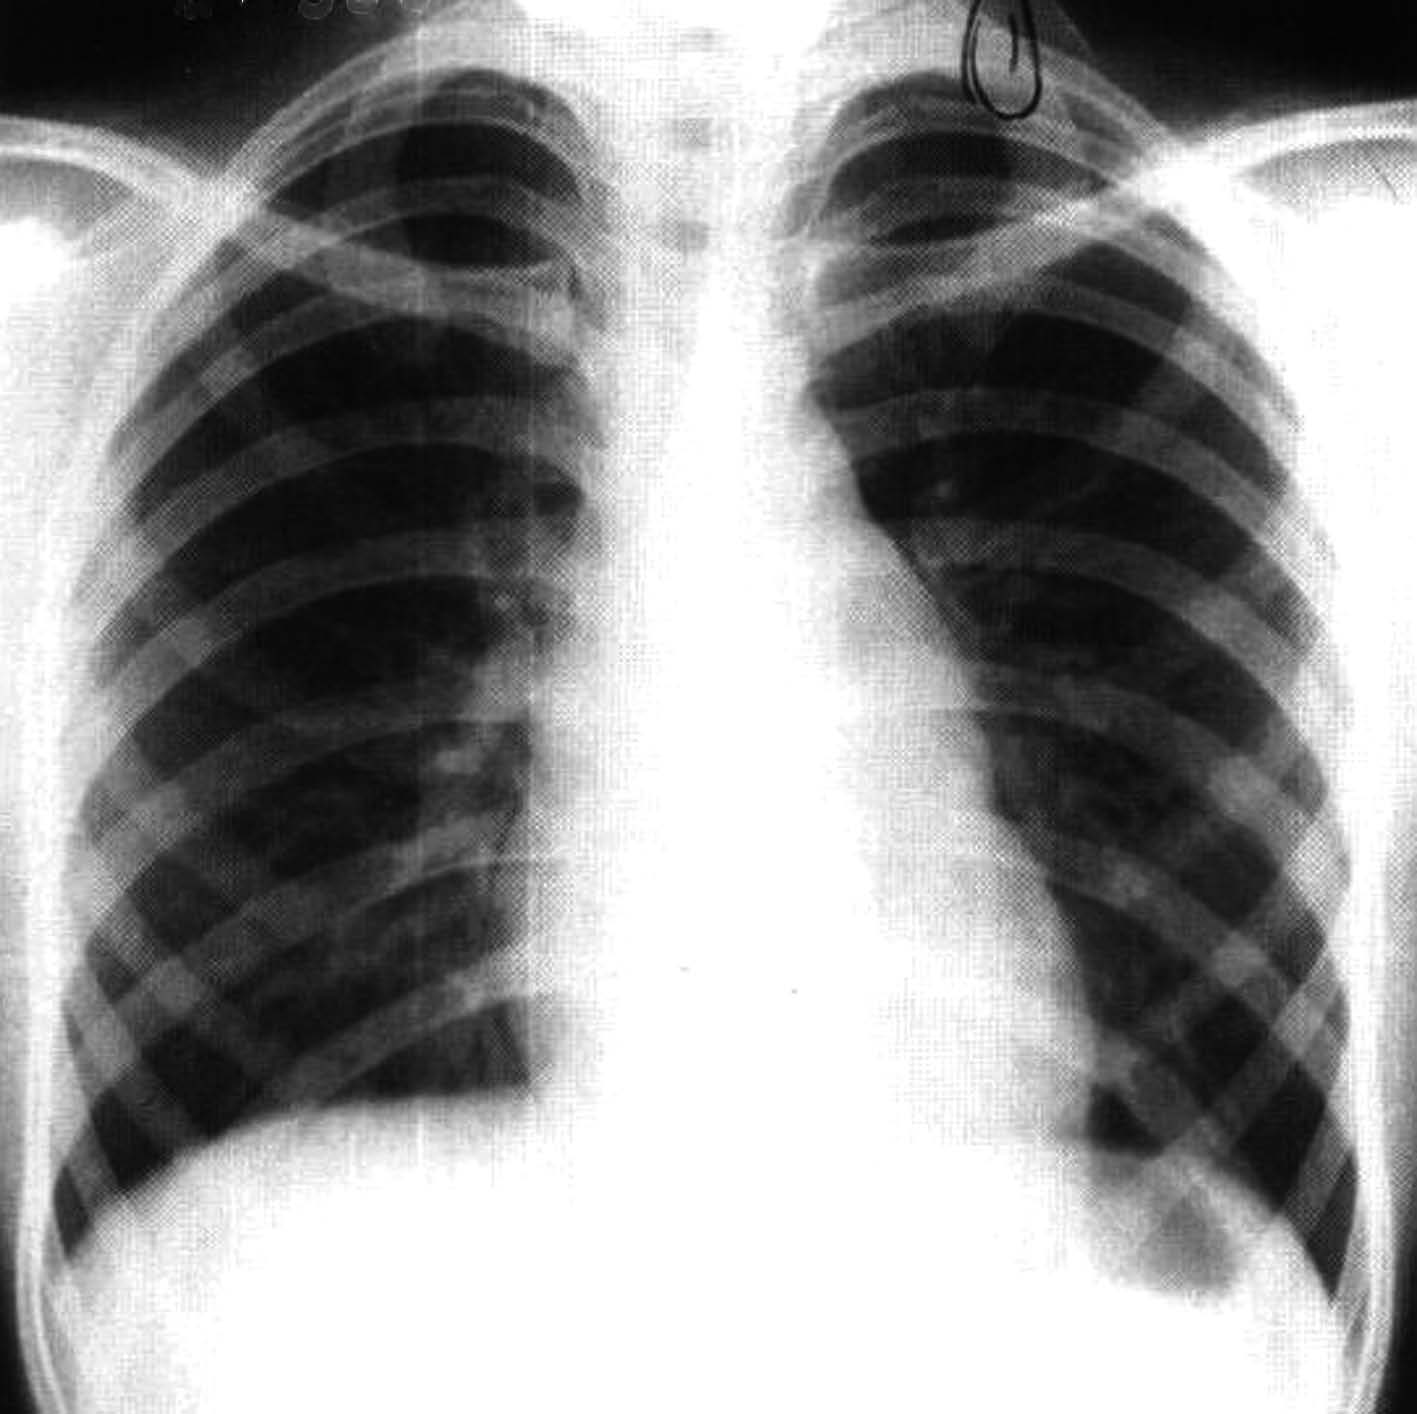
\includegraphics{./images/Image00219.jpg}
 \captionsetup{justification=centering}
 \caption{正位X线胸片,法洛三联症}
 \label{fig4-2-6}
  \end{figure} 

\textbf{【病史摘要】}
 女性,11岁。气喘且时有蹲踞6年,近两年来口唇有轻度发绀。听诊:胸骨左缘第2至第3肋间闻有Ⅵ级收缩期杂音。

\textbf{【X线表现】}
 主动脉结小,肺动脉段突隆,心左缘圆隆,心影呈梨形改变,心胸比率0.46。两肺血管纹理略减少,左肺门影大于右肺门影,右下肺动脉影不增宽。

\textbf{【X线诊断】}  法洛三联症。

\textbf{【评  述】}
 肺动脉狭窄,主要是瓣膜狭窄可伴卵圆孔未闭或心房间隔缺损(绝大多数为二孔型)。这种合并畸形有两种情况:一种情况是肺动脉狭窄较重,右心的排血阻力超过左心,于心房水平形成右向左或双向分流,临床上可出现发绀,再加继发的右心室肥厚,常称为法洛三联症。心房间分流的病理基础最多是卵圆孔未闭,而在血流动力学上起主导作用的是重度肺动脉瓣狭窄;另一种情况是心房水平为左向右分流,临床上无发绀,病理多为二孔型房间隔缺损,而肺动脉狭窄较轻。显然应与上述的三联症有所区别,称为房间隔缺损合并肺动脉瓣狭窄更为恰当。肺血正常或增多,与二孔型房间隔缺损相似。

三联症X线平片所见与典型的肺动脉瓣狭窄无异,结合临床出现发绀即可诊断,本例均符合之。个别病例可为漏斗部狭窄合并瓣膜狭窄,这种情况与法洛四联症不易鉴别,需行心室造影助诊。

\subsection{三尖瓣下移畸形}

\begin{figure}[!htbp]
 \centering
 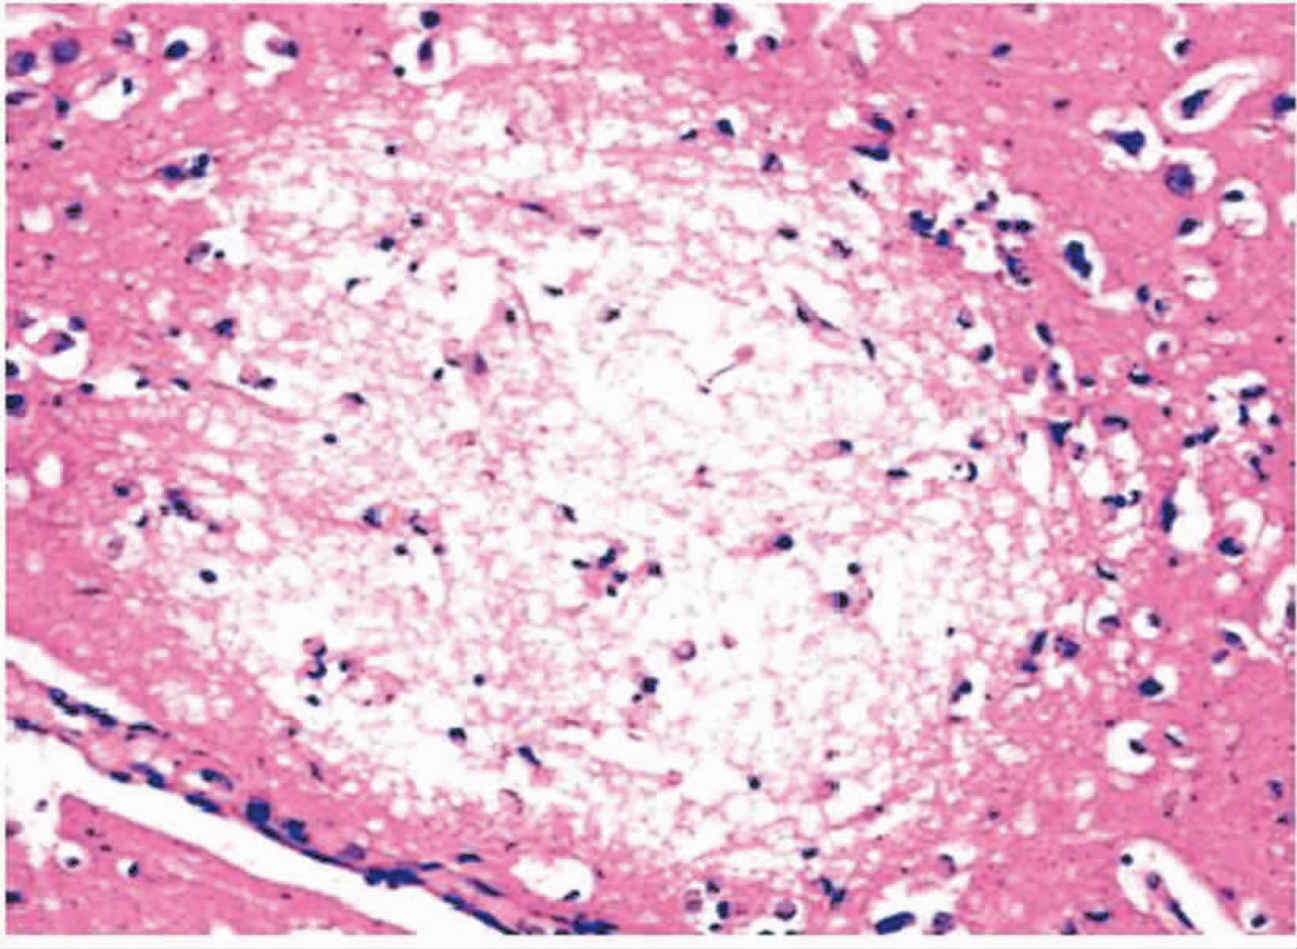
\includegraphics{./images/Image00220.jpg}
 \captionsetup{justification=centering}
 \caption{正位X线胸片,三尖瓣下移畸形}
 \label{fig4-2-7}
  \end{figure} 

\textbf{【病史摘要】}
 女性,10岁。气短伴轻度发绀5年余。听诊:心前区听到Ⅵ级收缩期杂音。心电图示右心房扩大肥厚及完全性右束支传导阻滞。

\textbf{【X线表现】}
 主动脉结小,心影显著向两侧增大。以左侧增大为主,心影呈烧瓶状,心右缘下段明显向右、向上膨隆突出,下段与上段比值为0.63。心底部大血管蒂影缩小,两肺纹理纤细稀疏,肺野透亮度增高,心胸比率为0.79。

\textbf{【X线诊断】}  三尖瓣下移畸形。

\textbf{【评  述】}
 三尖瓣下移畸形并非罕见,右房室环位置正常,一般三尖瓣前尖(前瓣)在正常位置,隔侧尖(隔瓣)和后尖(后瓣)下移附着于心室内壁,如是右心被分成一巨大的心腔和具有右心室功能的流出道。房化的右心室流入道不与右心房而与右心室同步收缩,收缩驱使血液向固有心房逆流,无效工作,右心房排空延迟,压力升高。多数病例并有心房间的异常通道(多为卵圆孔未闭)。

根据病理及血流动力学改变,主要X线征象为心脏多呈中至高度增大,外形如烧瓶或球形,本病特殊表现为巨大右心房,心底部大血管蒂影缩小,肺少血改变,临床有轻度发绀,为典型三尖瓣下移畸形。本病有别于常见肺少血的以右心室肥厚增大的肺动脉狭窄、法洛三联症、法洛四联症,因其均无巨大右心房,无心底部大血管蒂影缩小,心影增大程度及外形亦不同。此外,尚需与限制性心肌病鉴别,后者主要表现为心尖部的挛缩,心脏超声检查或心血管造影可以明确诊断。

\section{风湿性心脏病}

\subsection{二尖瓣狭窄}

\begin{figure}
  \centering
\subfloat[正位X线胸片,风湿性心脏病二尖瓣狭窄]{
\begin{minipage}[b]{0.48\textwidth}
\centering
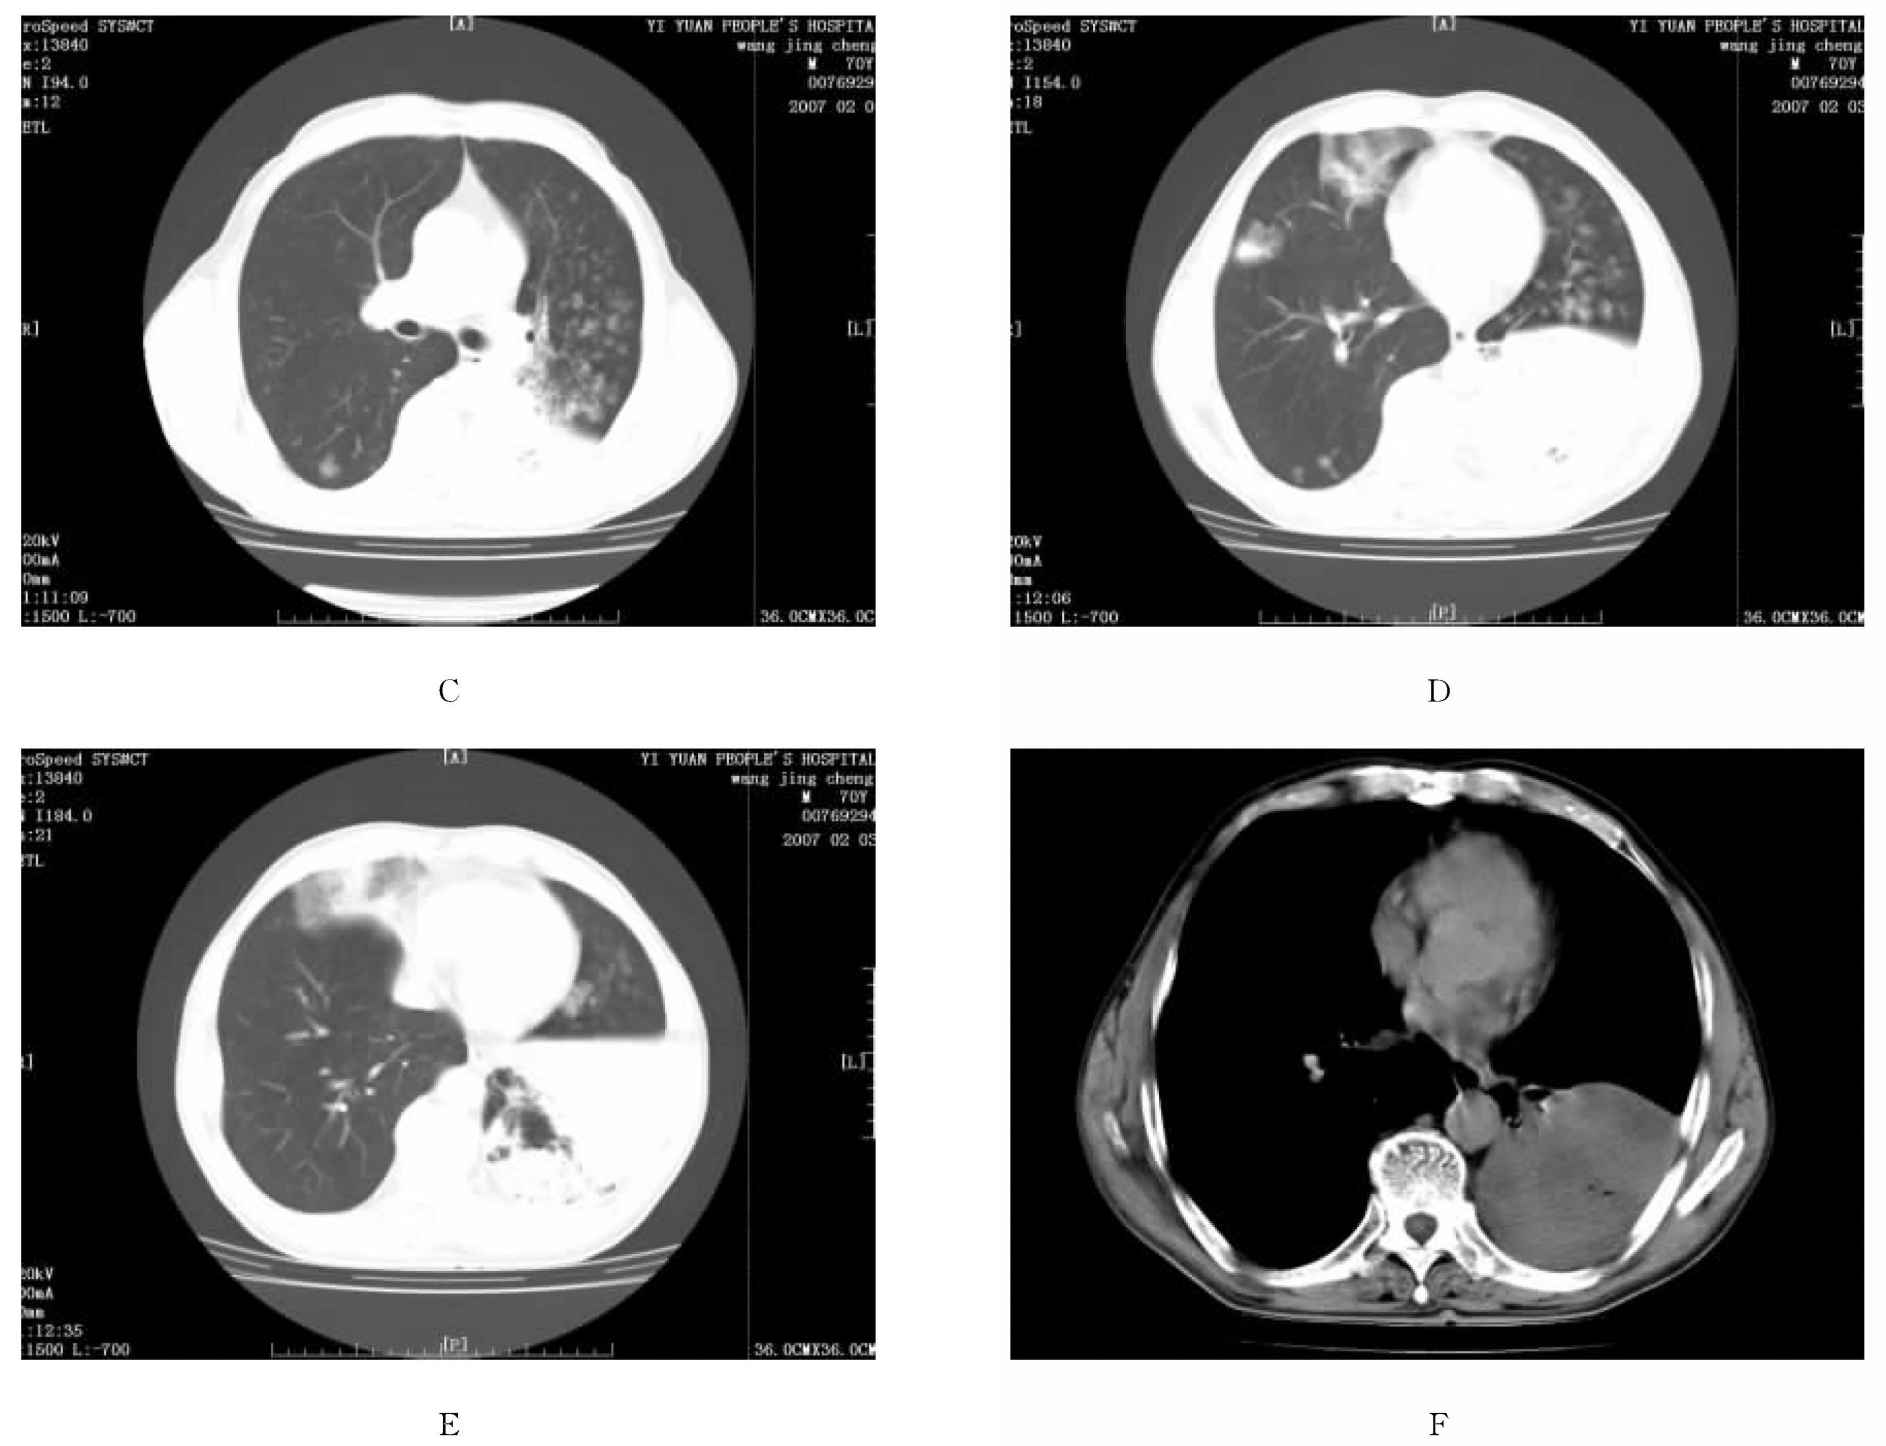
\includegraphics[height=.36\textheight]{./images/Image00221.jpg}
\end{minipage}}
\subfloat[同一患者右前斜位吞钡X线胸片]{
\begin{minipage}[b]{0.48\textwidth}
\centering
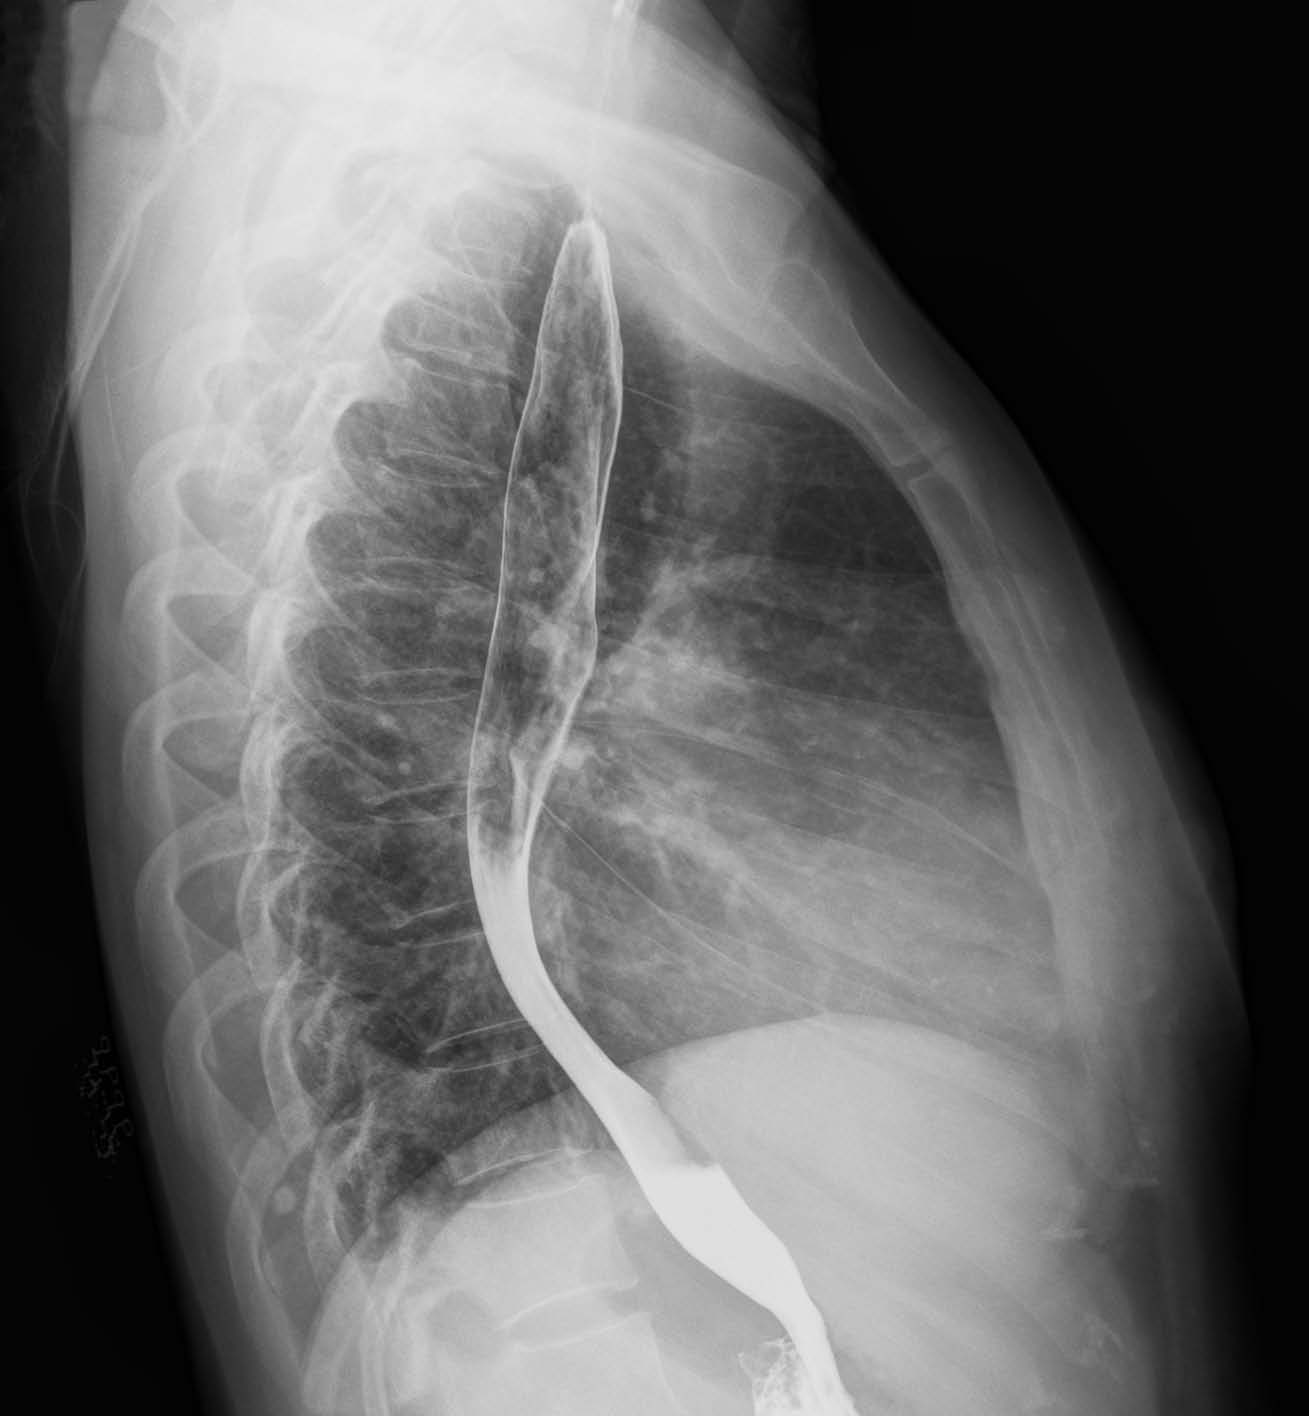
\includegraphics[height=.36\textheight]{./images/Image00222.jpg}
\end{minipage}}\\
\caption{}
\label{fig4-3-1}
\end{figure}

\textbf{【病史摘要】}  女性,37岁。发现心脏杂音20年,胸闷、气短3年余。

\textbf{【X线表现】}
 正位X线胸片示心影呈梨形,主动脉结缩小,肺动脉段突出,右下肺动脉稍增粗,右心缘双房影,左心缘见第三弓,心膈接触面增大,心尖向左下移。两肺纹理增多,边缘模糊。右前斜位吞钡X线片示食管中下段局限性向后压迫移位,心前间隙缩小。

\textbf{【X线诊断】}  风湿性心脏病二尖瓣狭窄。

\textbf{【评  述】}
 风湿性心脏病(简称风心病),包括急性或亚急性风湿性心脏病及慢性风湿性瓣膜病两大类。后者各瓣膜均可受累,以二尖瓣最为常见。多数发生于心脏左侧,于右侧者常与左侧同时并发,其中最多见于二尖瓣,其次为主动脉瓣,其他瓣膜损害比较少见。二尖瓣狭窄所致的梨形心较典型。本病女性多于男性。常有心悸、气短、胸痛及咯血等,也可出现发绀及急性肺水肿。体格检查以二尖瓣面容、心尖部舒张期隆隆样杂音为特征,可触及震颤。心电图示二尖瓣P波,右心室肥厚及劳损以及右束支传导阻滞等。X线平片检查可以初步判定瓣膜受损的部位、性质狭窄和(或)关闭不全及其严重程度。

病理生理改变:二尖瓣发生狭窄,左心房收缩时血液排空进入左心室发生障碍,造成左心房内的血量增加、郁积,使左心房压力升高,左心房逐渐扩大和肥厚;由于左心房压力升高,肺静脉及肺毛细血管压力也同时升高,肺静脉及肺毛细血管扩张瘀血,这时肺动脉压必须上升,才能保持正常的肺动脉与肺静脉压差,保持有效的肺循环,致使右心室增加负荷,逐渐肥厚;长期肺静脉循环阻力增高,进而引起肺动脉高压,促使右心室肥厚扩大;长期二尖瓣狭窄,左心室血流量减少,左心室及主动脉都可以有萎缩改变。

二尖瓣狭窄的心脏X线表现:心脏增大的大小可从轻度到显著,一般为中度增大,外形通常呈梨形或称二尖瓣型心脏。左心房增大是二尖瓣狭窄最主要的和最常见的X线征象。后前位上,心右缘可见到双重阴影或出现双弧影,心左缘左心耳增大,出现第三弧膨出,呈驼峰样;左、右支气管分叉角增大,尤其左侧支气管受压抬高。右前斜位吞钡,食管呈不同程度受压移位,依其程度将左心房增大分为轻、中、重三度;左前斜位吞钡,食管受压移位,主动脉窗缩小或消失,左侧支气管抬高。左侧位上,对确定左心房增大更有利。右心室增大为仅次于左心房增大的重要征象,是肺内压力增高的结果,因此常伴有肺动脉高压的存在。轻度二尖瓣狭窄右心室增大常不显著,重度二尖瓣狭窄右心室呈中度以上增大。后前位上,表现心向左旋转,肺动脉段突出,心脏横径加宽,心尖上翘圆钝;左、右斜位,心脏前下缘向前膨凸,心前间隙缩小或消失。右心房增大在二尖瓣狭窄中比较少见,绝大多数是轻度增大,多是相对性三尖瓣关闭不全或右心衰竭,较明显的右心房增大常提示有三尖瓣损害。因左心房流入左心室的血量减少,左心室发生萎缩而缩小。左前斜位上,心后缘下段变短前缩与增大后凸的左心房形成鲜明的对比。由于左心室进入主动脉的血量减少和右心室增大使心脏向左旋转,造成主动脉升、降部重叠,使主动脉结缩小。病变后期,二尖瓣可出现形态不规则的钙化,从而进一步影响二尖瓣的功能。

二尖瓣狭窄的肺部X线表现:肺血管纹理增多、交叉成密集的网状阴影、肺野透亮度减低、肺底板模糊等肺瘀血改变,这是二尖瓣狭窄中的重要征象。重度肺瘀血可产生小叶间隔水肿,出现Kerley氏B线,在肺的下部、肋膈角区最多见,呈水平横行条影,长2~3cm,宽1~2mm,数条平行,可双侧同时出现,也可单侧出现。由于肺静脉压力升高,逐渐出现上肺静脉增粗、下肺静脉变细的现象,这种改变主要是由于压力升高而引起下叶血管反射性收缩所致。后期肺内可出现许多细小如粟粒样颗粒,为含铁血黄素沉着所致。随着肺静脉压力的持续升高,引起肺毛细血管、肺小动脉压力的升高,最后导致肺动脉高压,其X线表现为:①肺动脉段凸出。②肺动脉主分支扩张,右下肺动脉干宽度超过15mm。③肺动脉主支扩大,而肺野外围分支出现骤然细小呈残根状。

X线诊断二尖瓣狭窄一般没有困难。典型的单纯二尖瓣狭窄根据病史及体征即可明确诊断。有时需与某些血流动力学相似的疾患鉴别,如左房粘液瘤、马方综合征(Marfan
syndrome)或室间隔缺损继发主动脉瓣关闭不全、主动脉瓣上或瓣下狭窄以及各种心肌疾患继发的二、三尖瓣关闭不全等。此时,需对全面资料尤其是超声心动图进行综合分析做出诊断。左心房粘液瘤病例的心脏杂音可能随体位变动而改变响度或消失。超声心动图可显示左心房内肿瘤的云团状回声反射,在舒张期进入二尖瓣瓣口或左心室,收缩期时回纳入左心房内,对明确诊断极有价值。考虑做外科手术治疗的二尖瓣狭窄病例,尚需查清是否伴有二尖瓣关闭不全及其他瓣膜是否也有病变以及病变的轻重程度。40岁以上的病例宜做选择性冠状动脉造影术以了解冠状动脉有无梗阻性病变。

\subsection{二尖瓣狭窄伴关闭不全}

\begin{figure}[!htbp]
 \centering
 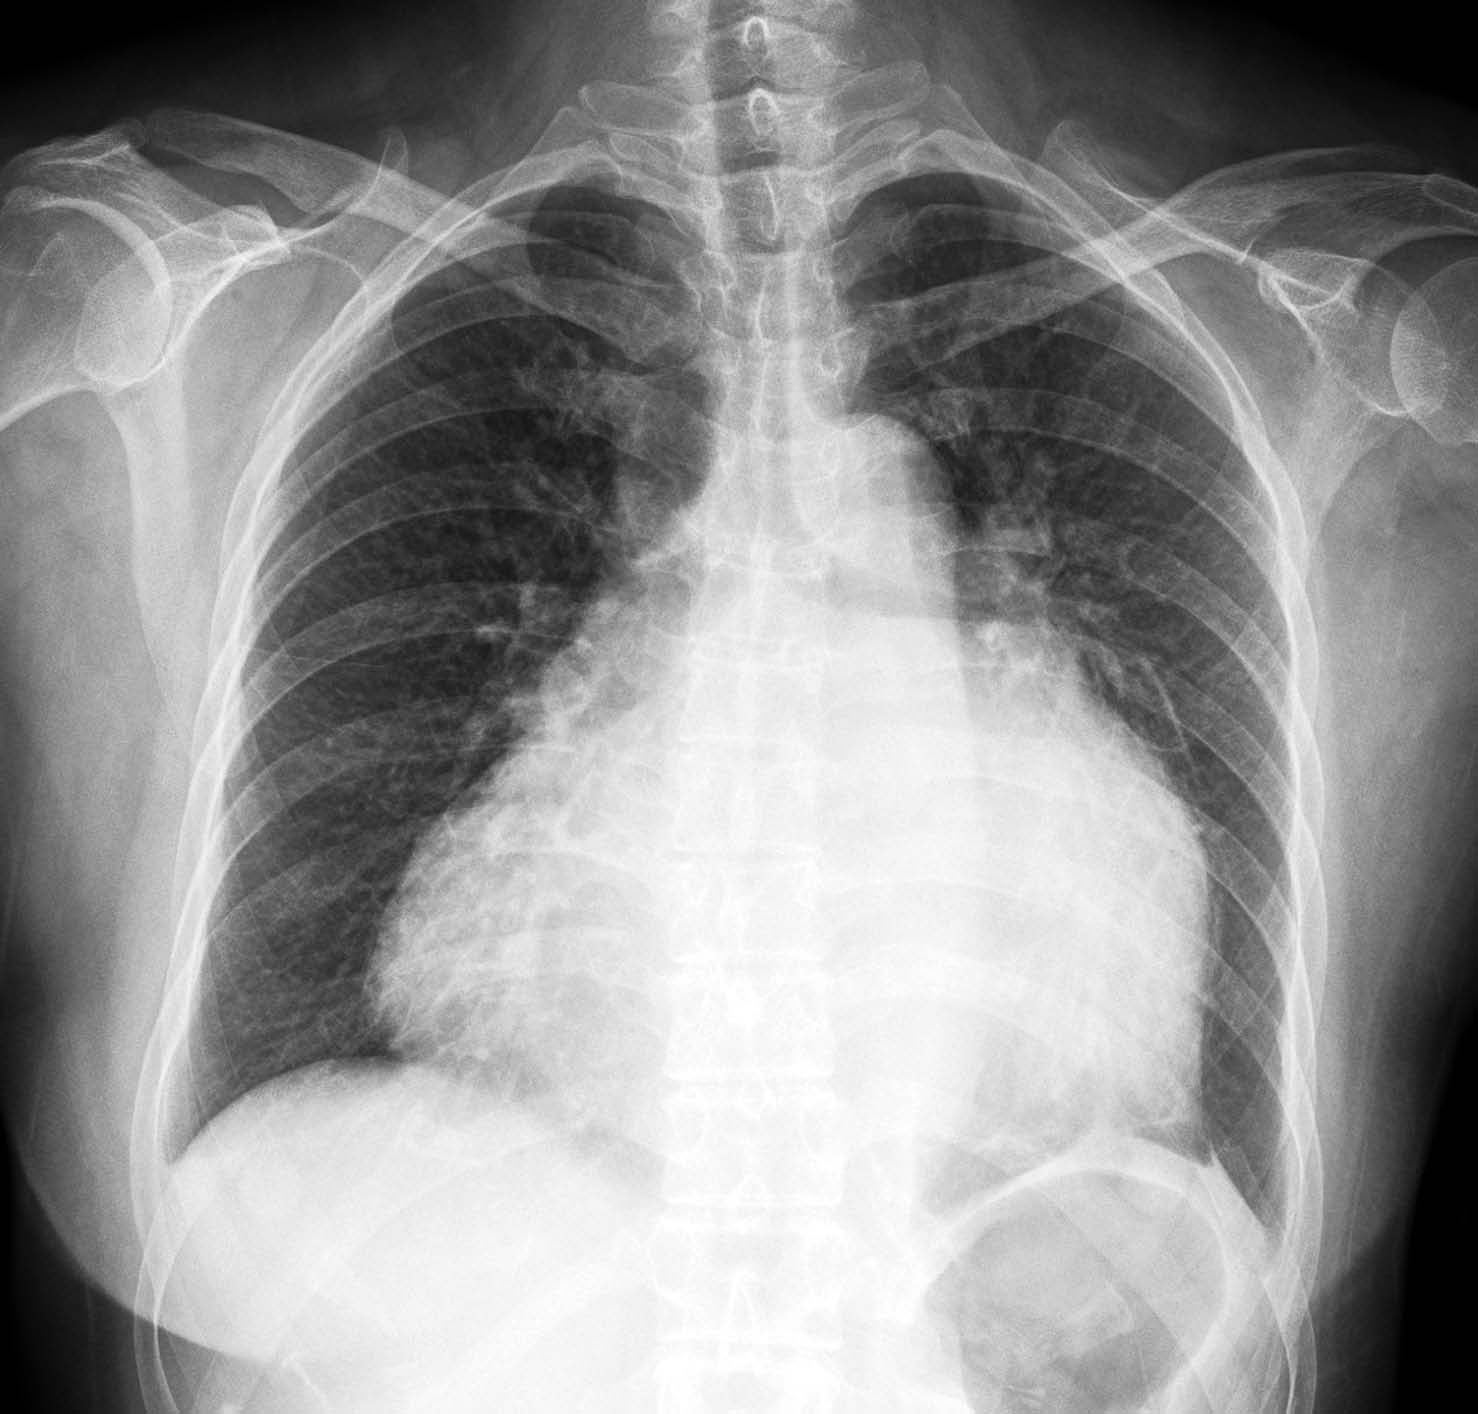
\includegraphics{./images/Image00223.jpg}
 \captionsetup{justification=centering}
 \caption{正位X线胸片,二尖瓣狭窄伴关闭不全}
 \label{fig4-3-2}
  \end{figure} 

\textbf{【病史摘要】}
 女性,55岁。活动后胸闷、气急5年余。体格检查:心尖区闻及Ⅵ级收缩期及响亮的舒张期杂音。

\textbf{【X线表现】}
 主动脉结小,肺动脉段稍突隆,心影向两侧增大,心左缘向左下延伸,食管明显向右移位,心右缘见双房影,心胸比率0.7。两肺门影增浓,两上肺静脉增粗,两下肺透亮度减低;左右支气管夹角明显增大,左支气管上抬。

\textbf{【X线诊断】}  风湿性心脏病:二尖瓣狭窄伴关闭不全。

\textbf{【评  述】}
 风湿热致二尖瓣瓣膜长期反复炎症,二尖瓣瓣膜纤维化、增厚、僵硬,交界融合,造成瓣口狭窄,同时瓣叶因纤维化挛缩变形,瓣口游离缘因纤维化增厚或钙质沉积卷曲不平整,致使前后瓣叶不能在心室收缩时对拢闭合,腱索乳头肌也因纤维化、短缩,将瓣叶向心室腔牵拉,以致瓣叶活动度受到限制,阻碍瓣膜的开闭功能,使二尖瓣既有瓣口狭窄,又有关闭不全。二尖瓣叶收缩变形和瓣膜组织的缺损(相对的和绝对的),使两瓣叶于收缩期末未能紧密闭合而产生关闭不全。结合血流动力学变化,左心房和左心室增大,而无明显的肺循环高压,尤其是肺动脉高压的征象。单纯二尖瓣关闭不全少见,多与二尖瓣狭窄合并存在。

二尖瓣狭窄伴关闭不全的X线征象:既具有二尖瓣狭窄的X线表现,同时又有左心室增大的表现。总之,二尖瓣狭窄时,有高度左心房增大、左心室增大及心影明显增大,应考虑合并二尖瓣关闭不全的存在。当有右心室增大、高度左心房增大、左心室增大、心影中度以上增大、有肺循环高压及肺瘀血,为典型二尖瓣狭窄伴关闭不全的X线表现。与联合瓣膜病变(常见的是二尖瓣狭窄+主动脉瓣关闭不全)的鉴别,后者常无高度左心房增大,心影多呈二尖瓣型或主动脉型,左心室增大较明显,主动脉缩小不显著,再结合心脏杂音则可鉴别。

\section{高血压性心脏病}

\subsection{高血压性心脏病}

\begin{figure}[!htbp]
 \centering
 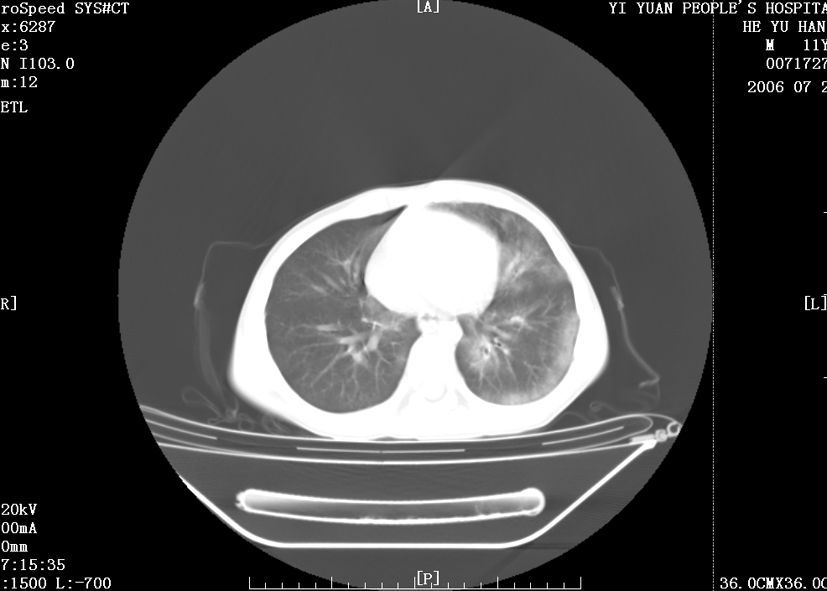
\includegraphics{./images/Image00224.jpg}
 \captionsetup{justification=centering}
 \caption{正位X线胸片,高血压性心脏病}
 \label{fig4-4-1}
  \end{figure} 

\textbf{【病史摘要】}
 女性,63岁。阵发性胸闷1个月。体格检查:血压164/102mmHg。

\textbf{【X线表现】}
 心影呈主动脉型,主动脉结突出,心腰凹陷,主动脉增宽迂曲,左心缘下段向左扩大,心尖左下移位。两肺纹理增多,边缘欠清晰。

\textbf{【X线诊断】}  高血压性心脏病。

\textbf{【评  述】}
 头痛、头晕、失眠是高血压的常见症状,在心功能代偿期一般无心脏方面的症状。发展至高血压性心脏病后可逐渐出现左心衰竭症状(心悸、气短、不能平卧、心动过速甚至出现奔马律、肺水肿等),如继发右心衰竭可见肝大、下肢水肿等相应表现。

高血压病可分为原发性和继发性两类,前者约占90%,后者10%,继发于其他疾病如肾脏、内分泌、心血管和颅脑疾患等。各型高血压达到一定时间和程度,使左心室负荷加重,继之引起左心室肥厚、增大和功能不全。

X线表现:典型者心脏呈“主动脉”型,主动脉增宽,主动脉结膨凸,左心室增大。单纯左心室肥厚,在后前位上仅表现左心室段圆隆,心尖钝圆,即所谓向心性肥厚,整个心影无明显增大。当左心室肥厚和扩张而引起左心室增大时,在后前位上,心脏呈主动脉型,左心室缘向左凸隆,并向下延伸,相反搏动点上移。左前斜位上,心脏向后凸出,心后间隙消失,与脊柱影重叠。后期致左心衰竭时,左心室发生显著增大,搏动减弱,可继发相对性二尖瓣关闭不全,因此,左心房、左心室进一步扩大,肺静脉压力升高,出现肺瘀血,以及间质性或肺泡性肺水肿。

心电图是诊断高血压引起的心脏改变的重要根据。一般来说左心室高电压、肥厚、劳损等与X线所示的心脏和左心室增大呈正相关关系。但有些病例心电图改变早于X线改变或X线改变早于心电图改变。因此,诊断高血压性心脏病应同时重视两个指标,相互配合。二维超声、CT、MRI除显示心脏改变外对主动脉缩窄、肾及肾上腺改变等继发性高血压的病因诊断具有重要价值。血管造影(包括DSA)对继发于主动脉缩窄、大动脉炎和肾血管病的高血压能提供最准确的解剖诊断,作为手术和介入性治疗的依据。一般来说,综合临床,心电图、胸片和二维超声做出高血压性心脏病的诊断较符合我国的国情。

\section{慢性肺源性心脏病}

\subsection{慢性肺源性心脏病}

\begin{figure}[!htbp]
 \centering
 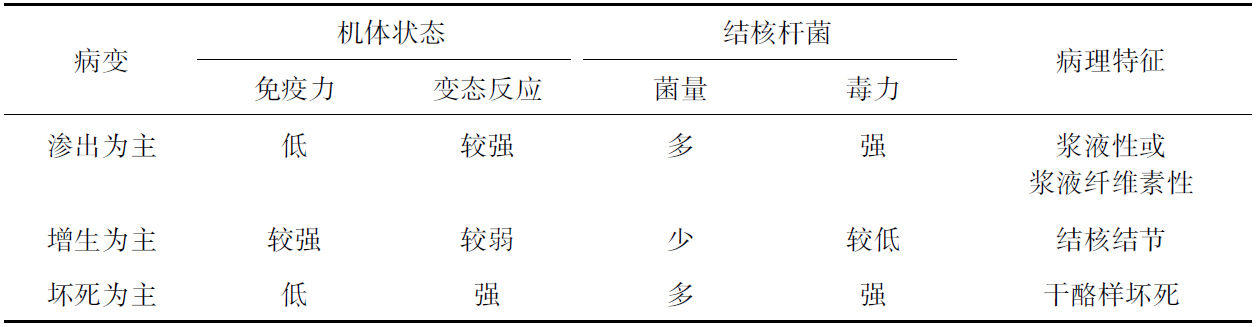
\includegraphics{./images/Image00225.jpg}
 \captionsetup{justification=centering}
 \caption{正位X线胸片,肺源性心脏病}
 \label{fig4-5-1}
  \end{figure} 

\textbf{【病史摘要】}  男性,56岁。反复咳嗽、气喘9年,加重4天。

\textbf{【X线表现】}
 两肺纹理增多、紊乱,两肺野增大及透亮度增加,右肺门旁见无肺纹泡状透亮影;右下肺动脉干增粗(最大横径大于15mm)呈残根样改变,肺动脉段突出,左心缘下段圆隆上翘。纵隔无增宽,两横膈低位。

\textbf{【X线诊断】}
 两肺慢性支气管炎肺气肿改变,右上肺大疱;肺动脉高压;肺源性心脏病。

\textbf{【评  述】}
 本病发展缓慢,临床上除原有肺、胸疾病的各种症状和体征外,主要是逐步出现肺、心功能衰竭以及其他器官损害的表现。对于慢性肺、胸疾患患者,最常见的是慢性支气管炎和肺气肿,其次是严重的肺结核、肺尘埃沉着症、支气管扩张以及广泛的胸膜增厚、胸廓畸形等,肺血管病变如肺动脉血栓栓塞等。肺动脉高压的X线表现有:①肺动脉主支扩大,以右肺下动脉扩张最明显,其横径大于15mm。②中心肺动脉扩张外围分支细小,两者形成鲜明对比,呈残根状,多反映较重度的肺动脉高压。③肺动脉段突出,与肺动脉高压程度及病程长短有关,早期仅轻度膨隆,严重时可明显突出。

慢性肺源性心脏病的心脏改变:由于有肺动脉高压,肺动脉段凸出,肺动脉主干搏动增强;右心室增大,心脏横膈接触面增宽,因此心脏外形如梨形,呈二尖瓣型。由于肺气肿,横膈低及心脏增大不显著,心胸比率大于正常者不多。部分病例心脏外形可比正常者为小(小肺心)。心脏代偿功能减退出现心力衰竭时,心脏可急骤增大,而当心力衰竭被控制后,心脏大小又可回复原状。右心房增大不多见,常由于右心室压力增高,右心房排血困难并发三尖瓣关闭不全而出现,故都与右心室增大并存。

慢性肺源性心脏病常需与冠状动脉粥样硬化性心脏病(冠心病)、风湿性心瓣膜病、原发性心肌病等相鉴别。肺心病与冠心病均多见于老年人,有许多相似之处,而且常有两病共存。冠心病有典型的心绞痛、心肌梗死的病史或心电图表现,若有左心衰竭的发作史、高血压病、高脂血症、糖尿病史更有助鉴别;体检、X线及心电图检查呈左心室肥厚为主的征象,可资鉴别;肺心病合并冠心病时鉴别有较多的困难,应详细询问病史,体格检查和有冠心病、肺功能检查加以鉴别。风湿性心脏病三尖瓣疾患应与肺心病的相对三尖瓣关闭不全相鉴别,前者往往有风湿性关节炎和心肌炎的病史,其他瓣膜如二尖瓣、主动脉瓣常有病变,X线、心电图、超声心动图有特殊表现。原发性心肌病多为全心增大,无慢性呼吸道疾病史,无肺动脉高压的X线表现等可资鉴别。

慢性肺源性心脏病的X线诊断:应根据肺部、心脏两方面改变进行全面分析,肺部病变是根本,肺动脉高压是线索,右心室增大是依据。肺动脉高压和右心室增大应做出明确的判断,是诊断早期肺心病的关键。

\section{冠心病}

\subsection{冠心病}

\begin{figure}[!htbp]
 \centering
 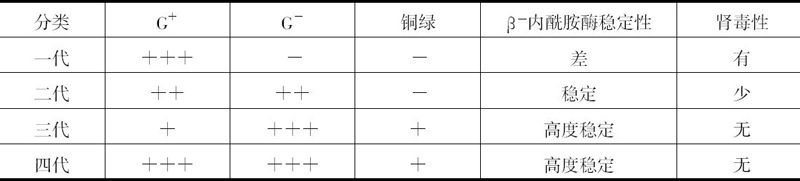
\includegraphics{./images/Image00226.jpg}
 \captionsetup{justification=centering}
 \caption{正位X线胸片,冠心病}
 \label{fig4-6-1}
  \end{figure} 

\textbf{【病史摘要】}
 男性,77岁。间断性剑突下及胸背痛1个月,疼痛呈间歇性发作,可忍受,发作持续5~10分钟,有高血压病史20年,规则服抗高血压药。体格检查:血压为146/92mmHg,心律齐,心界扩大。

\textbf{【X线表现】}
 两肺纹理增多,两肺野内未见明显异常密度影,两肺门影正常;主动脉影增宽迂曲,主动脉管壁可见弧状高密度钙化影,心影增大,呈靴型外形,心尖向左下延伸。

\textbf{【X线诊断】}  结合病史考虑:冠心病。

\textbf{【评  述】}
 由于脂质代谢不正常,血液中的脂质沉着在原本光滑的动脉内膜上,形成一些分散的类似粥样的脂类物质堆积而成的白色斑块,称为动脉粥样硬化病变。这些斑块渐渐增多造成动脉腔狭窄,使血流受阻最终产生栓塞。动脉壁的病变发展下去斑块可能形成溃疡,还可并发血栓,造成血流阻断,相应组织细胞发生缺血性坏死。如果粥样硬化病变发生在冠状动脉引起心肌细胞缺血、缺氧,甚至坏死,继而引起的心脏病,这便是冠状动脉粥样硬化性心脏病。

根据冠状动脉管腔的狭窄及阻塞程度、发病的急缓、分布的范围和侧支循环形成的情况,可引起所属区域的不同程度的心肌缺血以致坏死,心脏和肺循环的X线征象也有很大的差异。隐性冠心病X线平片心脏大小、形态多无异常发现,心肌梗死可有左心衰竭、肺水肿、左心室增大、左心缘局限性搏动减弱或消失等。也可出现心肌梗死后综合征:包括心肌炎、胸膜炎和肺实质炎为其三主征。急性心肌梗死后或陈旧性梗死可有心室壁瘤出现。

患者无高血压病史,经临床已明确诊断为心肌梗死,心影轻度增大,左心室向心性肥厚,左心缘局限性搏动减弱,有间质性肺水肿及肺炎,上述X线表现支持冠心病诊断。

X线胸片对病情判断和预后评估有重要意义,对某些器质性并发症如心室壁瘤、室间隔穿孔(破裂)以及乳头肌功能失调或断裂的诊断也有一定的帮助。冠状动脉造影(含左心室造影)目前仍是诊断冠心病、选择冠心病患者手术和介入治疗适应证的可靠方法,显示冠脉及其分支的解剖形态、病变部位和病变程度。磁共振成像、多层螺旋CT冠状动脉造影是无创的检查技术,对冠状动脉狭窄(>50%)和冠状动脉搭桥术后桥血管阻塞的诊断、冠脉狭窄介入治疗适应证的选择,以及介入和手术治疗后的随访及其疗效的观察,都有初步的和良好的价值。超声心动图是诊断冠心病不可缺少的手段,它以简便、无创、重复性好而广泛应用于临床诊断、术中观察、术后及药物治疗评价等方面。核素心肌灌注显像是筛选冠状动脉造影最有价值的无创性手段;负荷心肌灌注显像阴性基本可排除冠脉病变,对心肌梗死、心肌梗死合并室壁瘤进行诊断以及评估存活心肌、评价血管重建术的疗效和冠心病患者预后等也是一项重要的检查手段。

\section{心肌病}

\subsection{心肌病}

\begin{figure}[!htbp]
 \centering
 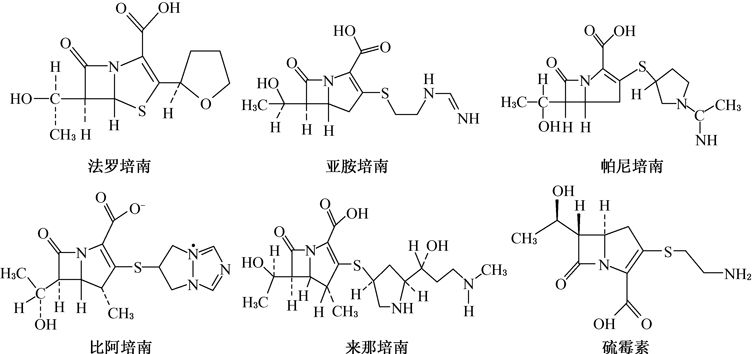
\includegraphics{./images/Image00227.jpg}
 \captionsetup{justification=centering}
 \caption{正位X线胸片,扩张型心肌病}
 \label{fig4-7-1}
  \end{figure} 

\textbf{【病史摘要】}
 男性,44岁。胸闷、活动后气急1个月余,有“扩张性心肌病”家族史。体格检查:血压为120/90mmHg,心律齐,心界扩大。

\textbf{【X线表现】}
 两肺纹理增多,边缘模糊,呈肺瘀血改变。心影呈主动脉型,主动脉结缩小,左心缘下段膨隆,心尖左下移位。右肋膈角钝。

\textbf{【X线诊断】}
 结合病史考虑:扩张型心肌病;两肺瘀血、右侧胸腔少量积液,提示左心功能不全。

\textbf{【评  述】}
 临床和病理学家将原因不明而又非继发于全身或其他器官系统疾病的心肌原发性损害定名为原发性心肌病。它是非风湿性、非高血压性、非冠状动脉性心肌结构和功能的病理改变。其病理过程属于代谢性而非炎症性,在发病机制上与其他已知病因引起的心脏病无关,是一组由于心脏下部分腔室(即心室)的结构改变和心肌壁功能受损所导致心脏功能进行性障碍的病变。相反,若心肌病变与已知病因有关,或继发或伴发于某种全身性疾病时,则称为继发性心肌病。原发性心肌病较少见,但分布于世界各地。对本病的概念、定义和病理变化等还有不同的认识,按病理可分为扩张型心肌病、肥厚型心肌病和限制型心肌病三种常见类型。其中以扩张型心肌病和肥厚型心肌病较为常见。

心肌病的发病原因至今未明。扩张型心肌病可能和某些因素如病毒、细菌感染或药物中毒导致代谢异常所致的心肌损伤有关,其中病毒性心肌炎被认为是最主要的原因。肥厚型心肌病可能与常染色体显性遗传有关,约1/3的有明显家庭史,儿茶酚胺代谢异常、高血压、高强度运动为其诱发因素。限制型心肌病以心内膜心肌纤维化、心肌僵硬及心室舒张充盈受阻为特征,多见于热带和温带地区,我国仅有散发病例。

一般起病缓慢,早期可有发热、乏力、头晕、气急等症状,晚期出现全心衰竭。心房颤动也较常见,心肌损伤和心肌的紧张或伸展常可导致心律失常(过快或过慢),部分可合并内脏栓塞。

扩张型心肌病X线表现:有两心室增大,以左心室扩大为著,左心室圆隆,向左、后突出,心影呈主动脉型;如伴有瓣膜受损,则可引起心房扩大,左心缘搏动减弱而不规则,而右心缘的搏动正常,甚至增强;肺动脉段无明显变化,有时可呈平直或稍丰满,肺血管的表现属正常范围;出现左心衰竭时,可见肺瘀血及间质性肺水肿,主动脉结正常或较小;如主动脉瓣狭窄时,可有升主动脉扩张;治疗后病情可好转,一般情况下扩大的心脏要恢复正常外形较难。肥厚型心肌病X线表现有心脏大小正常或增大,心脏大小与心脏及左心室流出道之间的压力阶差呈正比,压力阶差越大,心脏亦越大;心脏增大以左心室肥厚为主,主动脉不增宽,肺动脉段多无明显突出,肺瘀血大多较轻,常见二尖瓣钙化;心室造影示心室腔缩小,肥厚的心肌凸入心室腔内。限制型心肌病因病变易侵及右心室,X线表现约70%的患者显示心胸比例增大,合并右心房扩大者心影可呈球形;左心室受累时常可见肺瘀血。个别患者尚可见心内膜钙化影。

X线检查结合心电图、心脏超声、心导管检查,并结合临床资料,有利于心肌病与风湿性心脏病、心包积液、高血压性心脏病、冠心病、先天性心脏病相鉴别。有时心内膜心肌活检是确诊心肌病的重要手段。

\section{心包炎}

\subsection{心包积液}

\begin{figure}[!htbp]
 \centering
 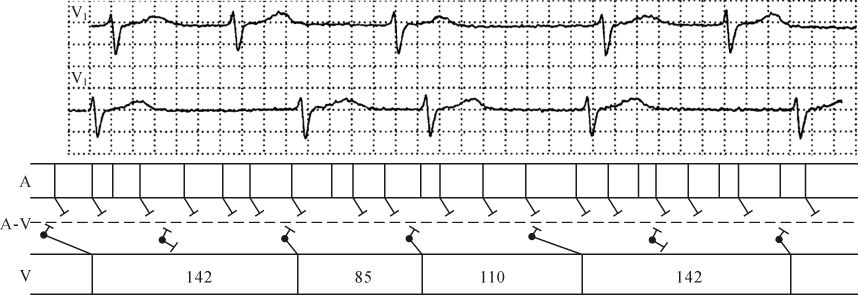
\includegraphics{./images/Image00228.jpg}
 \captionsetup{justification=centering}
 \caption{正位X线胸片,心包积液}
 \label{fig4-8-1}
  \end{figure} 

\textbf{【病史摘要】}
 女性,34岁。患尿毒症3年,加重1个月,常感呼吸困难。

\textbf{【X线表现】}
 两肺纹理增多,纹理边缘尚清晰。心影增大呈烧瓶样,心影各弓影分界不清。双侧肋膈角尚清。

\textbf{【X线诊断】}  结合病史考虑:尿毒症性心包炎,心包积液。

\textbf{【评  述】}
 临床上共同的特征是气短与胸部郁闷感,大量心包积液可出现心前区持久性压迫性疼痛,严重的呼吸困难。心尖搏动微弱或不能触及,心浊音界向两侧扩大,脉搏细速,动脉压下降,静脉压上升,脉压缩小,并可出现奇脉,有心包填塞征。颈静脉怒张,进行性肝大,心动过速。动脉压如持续下降,可引起休克。

急性心包炎时,临床闻及心包摩擦音即可确立诊断,但X线检查可无异常表现。成人积液少于250ml,儿童少于150ml,X线上多难识别。有学者提到心外脂肪征(Epicardial
fat
sign)有助于诊断心影正常的心包积液,侧位上正常心包为一线状致密影,其前方为密度低的纵隔脂肪,后方为心外脂肪;若侧位片上心包厚度超过2mm可诊为心包积液。正位上与侧位相似,但发现率较低。

积液量达300~500ml或以上时,X线上有一定的特征,心影中度或中度以上增大;心影各弓影分界不清,心影常向两侧呈球形或烧瓶状增大,心膈角可依心影形态的不同而异,球形者心膈角多锐利,烧瓶状者其心膈角可以变钝;透视下心影边缘搏动减弱或消失;主动脉搏动可以正常,但有心包填塞者,主动脉的搏动则减弱;卧位时心底部增宽及搏动减弱是诊断心包积液有意义的征象;上腔静脉影像增宽;短期复查心影变化大也支持心包积液的诊断。

心包积液的病因很多,有感染性、非感染性、代谢障碍性、肿瘤性心包炎等。虽然临床上由于起病的原因不同、分类亦颇多,但X线的检查为综合性的心包积液表现,而无法确定心包积液的性质和类型。超声心动图、MRI及CT对心包积液的诊断有很高的价值。对于少量心包积液,超声心动图更具有敏感性。核素显像与X线平片检查同样具有特异性,核素血池显像对大量心包积液与心脏增大的鉴别更有价值。

\subsection{缩窄性心包炎}

\begin{figure}[!htbp]
 \centering
 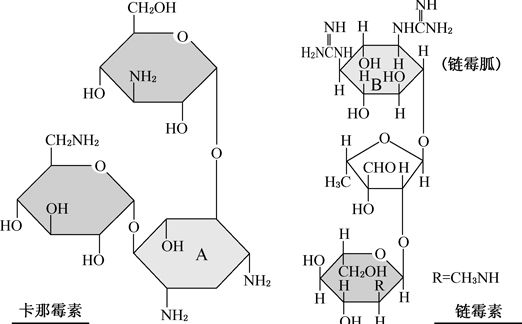
\includegraphics{./images/Image00229.jpg}
 \captionsetup{justification=centering}
 \caption{正位X线胸片,缩窄性心包炎}
 \label{fig4-8-2}
  \end{figure} 

\textbf{【病史摘要】}  女性,53岁。头晕1年,气喘、胸闷20多天。

\textbf{【X线表现】}
 两肺野清晰,未见明显异常密度影;心影大小、形态可,心脏膈面及右侧心包膜见线样钙化影,上腔静脉影明显增宽。

\textbf{【X线诊断】}  缩窄性心包炎。

\textbf{【评  述】}
 常有心悸、呼吸困难、胸闷等。体格检查见颈静脉怒张、肝大、腹水、下肢水肿、脉压差小、奇脉等。心电图示低电压、T波倒置、低平,有时可有房颤。X线表现心脏外形和大小基本正常或轻、中度扩大,心脏边缘呈不规则或僵硬,可呈天幕状改变,使正常心脏的弧度消失,心影似三角形或梨形;如局限性增厚,心缘可呈局限性突出;若与邻近组织发生粘连,可使心缘呈不规则或多边状。心脏及大血管的搏动明显减弱或消失,也可能造成不规则的搏动(无粘连部位搏动仍可见到,甚至明显增强),而主动脉的搏动减弱。上纵隔阴影增宽,肝脏增大,右膈升高,肺野有轻度瘀血。在左心缘有缩窄时,可出现间质性肺水肿及左心房增大,如二尖瓣狭窄则可出现一侧或两侧胸腔积液。增厚与粘连的心包膜可钙化,表现为蛋壳状或不规则影,累及整个心缘或其大部,在切线位上更明显。食管可由于粘连而产生移位,需注意不应与风湿性心脏病二尖瓣疾病相混淆。心脏改变轻微者,易发生漏诊。心脏增大者常应与心包积液、心肌病等区别。少数病例尚应与二尖瓣损害相鉴别。

心脏瓣膜疾病:局限性心包缩窄由于缩窄部位局限于房室沟和大血管出入口,可产生与瓣膜病及腔静脉阻塞病相似的体征。如缩窄局限于左房室沟,形成外压性房室口通道狭窄,体征及血流动力学变化酷似二尖瓣狭窄。风湿性心脏病二尖瓣狭窄可有风湿热史而无心包炎病史。心脏杂音存在时间较久。超声心动图示二尖瓣增厚或城墙样改变,瓣膜活动受限与左心室后壁呈同向运动。胸部X线检查,心脏搏动正常无心包钙化。心导管检查,缩窄性心包炎有特征性的压力曲线,再结合心血管造影有助于与先天性或后天获得性瓣膜病鉴别。

限制型心肌病:原发性或继发性限制型心肌病,由于心内膜和心肌受浸润或纤维瘢痕化,心肌顺应性丧失引起心室舒张期充盈受限。血流动力学和临床表现与缩窄性心包炎相似,鉴别诊断极为困难。因两者治疗方法、预后截然不同,故鉴别诊断很重要,确实难以鉴别时可采用开胸探查明确诊断。缩窄性心包炎为急性心包炎的后遗症,由于心包膜上有不同程度与范围的瘢痕和粘连,是形成粘连性心包炎和缩窄性心包炎的结果。由于粘连程度不同,造成对心脏功能的障碍亦不同。结核性心包炎因纤维组织增生显著,心包膜两层发生严重的增厚与粘连,因而形成坚厚的瘢痕。增厚的心包膜可局限性或弥漫性,严重的甚至可以完全闭塞心包腔,使心脏的收缩和舒张功能完全丧失,从而影响了静脉血回流到右心房,致使静脉压增高,颈静脉怒张,增厚的心包膜可产生钙化,呈一个盔甲心包。

MRI、CT及超声心动图对缩窄性心包炎的诊断有重要价值。平片检查亦具有较高的敏感性。对于不典型病例,以及与限制型心肌病的鉴别诊断上,MRI优于超声心动图。

\section{主动脉病变}

\subsection{主动脉窦瘤}

\begin{figure}[!htbp]
 \centering
 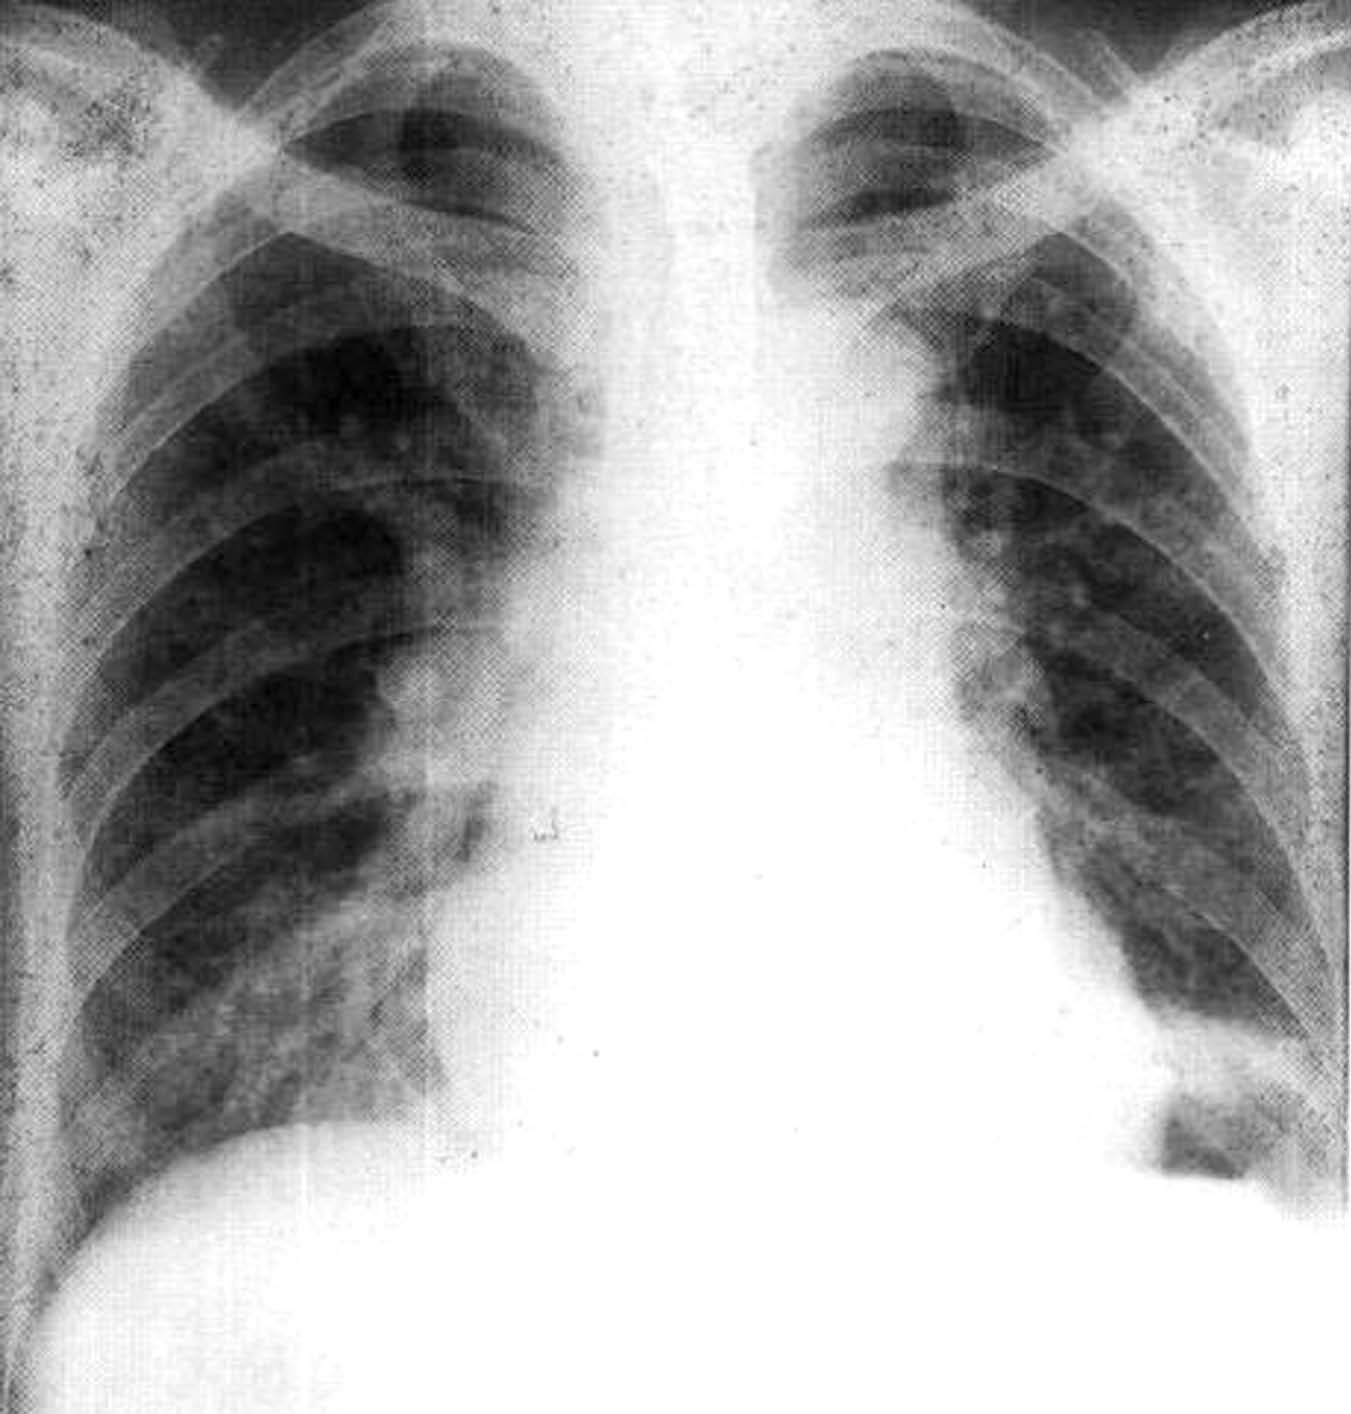
\includegraphics{./images/Image00230.jpg}
 \captionsetup{justification=centering}
 \caption{正位X线胸片,主动脉窦瘤破裂}
 \label{fig4-9-1}
  \end{figure} 

\textbf{【病史摘要】}
 男性,48岁。突然用力后心慌、气短伴左侧背痛3天入院。听诊:心前区及胸骨左缘第3至第4肋间可触及轻微震颤伴有Ⅳ级连续性杂音。心电图示左心室高电压。

\textbf{【X线表现】}
 主动脉影增宽,主动脉结增大,肺动脉段平直,心影稍向两侧增大,心影呈主动脉型,心胸比率0.6,两下肺纹理显著增粗、增多。

\textbf{【X线诊断】}  主动脉窦瘤破裂。

\textbf{【评  述】}
 主动脉窦瘤又称Valsalva's窦瘤,分先天性和后天性两种。一般认为先天性主动脉窦瘤系胚胎期主动脉根部中层弹力纤维的发育缺陷,未能与主动脉瓣的纤维环融合,形成局部管壁的薄弱区,加之主动脉内血压的影响,逐渐形成主动脉窦瘤或窦的憩室样膨突;后天性主动脉窦瘤是由于动脉壁中层坏死、心内膜炎、动脉粥样硬化、外伤、梅毒等因素所致。窦瘤一旦破入右心者构成心底部左向右分流。大多数窦瘤起源于右冠窦,少数起源于无冠窦,极少数起源于左冠窦。

本病少见,X线平片缺乏特征,又由于可合并各类畸形,X线表现可能以后者为主,更使平片诊断困难。此外,此类畸形临床常可闻及连续性杂音,尚易误诊为动脉导管未闭、主肺动脉隔缺损等病变。窦瘤破入右心后,则具有相当特征性的左向右分流X线征象,心影多呈中高度增大,左右心均受累,尤其是左心室增大为主,心影近似“主动脉”型,大多有肺血增多;少数有肺瘀血、间质性肺水肿等左心衰竭征象、心缘和主动脉搏动增强等。如熟悉上述较典型的X线表现,密切结合临床,平片诊断及其与常见的动脉导管未闭的鉴别并不困难。过去无心脏病的症状和体征,而成年后突然发病,并迅速出现心力衰竭则诊断更为确切。

X线心脏平片表现结合临床表现和体征可提示主动脉窦瘤诊断,详细的解剖诊断或与其他心底部分流、室间隔缺损合并主动脉瓣关闭不全的鉴别,则需要进一步的检查。超声心动图简便易行,特别是彩色多普勒技术对该病诊断的正确率可达95.5%,故应为本病首选检查方法。MRI对本病的诊断率随着MRI软、硬件技术的改善,定会不断提高,其优势为图像分辨率高,更符合解剖学所见,为手术治疗提供更直观信息。超声心动图诊断困难时,辅助MRI检查有助于提高诊断和鉴别诊断水平。胸主动脉造影检查是诊断该病的“金标准”。

\subsection{胸主动脉瘤}

\begin{figure}
  \centering
\subfloat[正位X线胸片,胸主动脉瘤]{
\begin{minipage}[b]{0.48\textwidth}
\centering
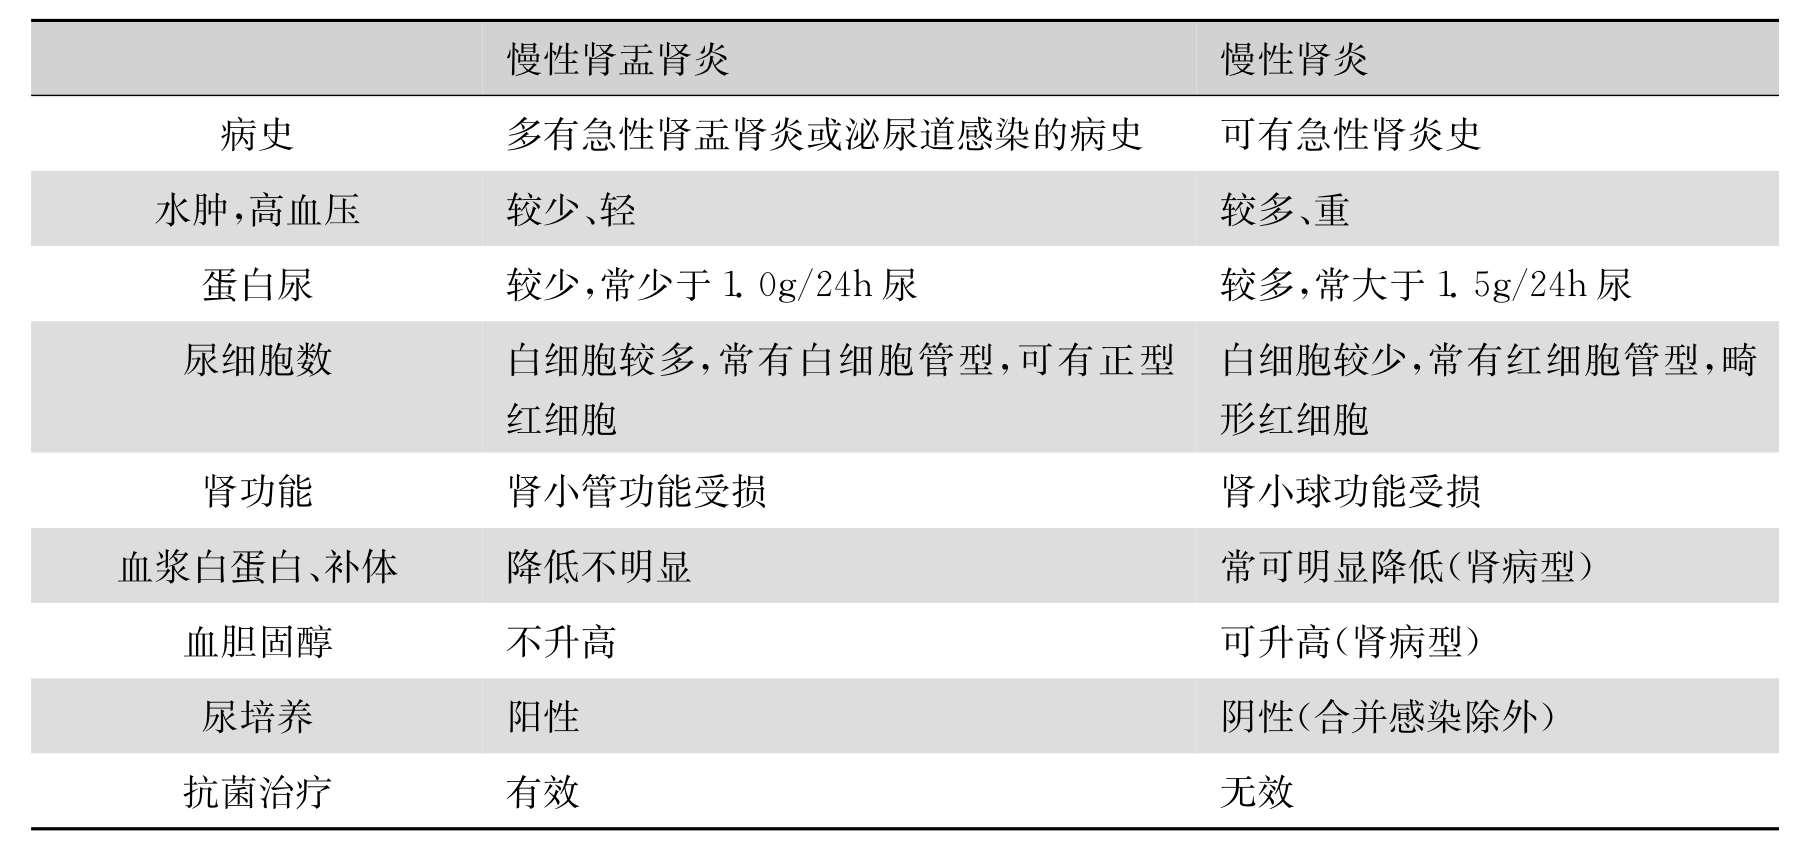
\includegraphics{./images/Image00231.jpg}
\end{minipage}}
\subfloat[CT多平面重建,胸主动脉瘤]{
\begin{minipage}[b]{0.48\textwidth}
\centering
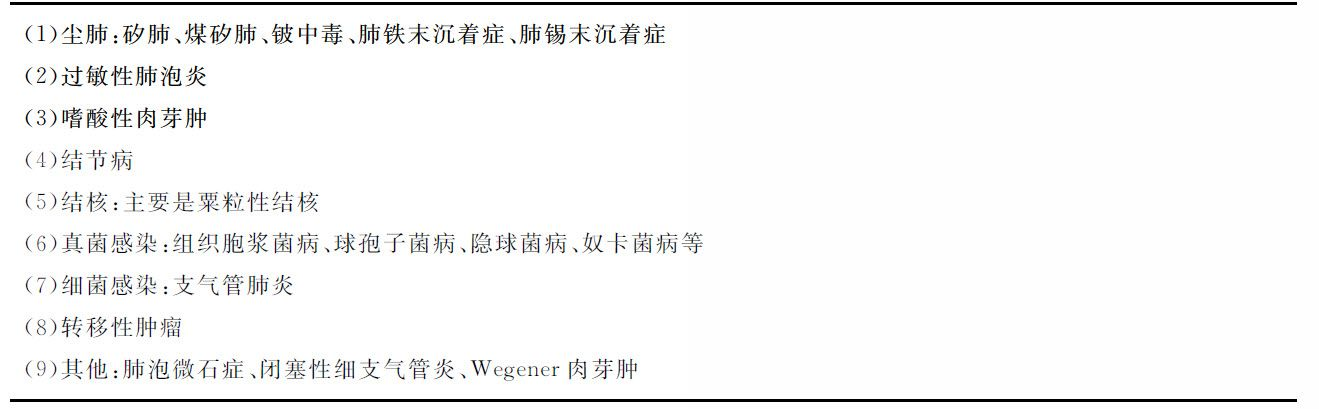
\includegraphics{./images/Image00232.jpg}
\end{minipage}}\\
\caption{}
\label{fig4-9-2}
\end{figure}

\textbf{【病史摘要】}
 男性,65岁。胸闷不适数年,近日突然用力后心慌、气短、胸痛入院。

\textbf{【X线表现】}
 后前位片示左中上纵隔(相当于主动脉弓处)有圆形块状阴影突入左侧肺野,密度均匀,轮廓光整,表面见散在斑块状钙化影,部分块影与心影重叠;两肺野清晰。CT胸主动脉血管造影最大密度投影成像示胸主动脉降段明显瘤样扩张,瘤内见低密度附壁血栓。

\textbf{【X线诊断】}  胸主动脉瘤伴瘤内附壁血栓。

\textbf{【评  述】}
 胸主动脉的病理性扩张称为胸主动脉瘤。虽病因各异但发病机制大致相似,主要是动脉壁中层弹力纤维断裂、中断,形成局部的薄弱区,加之动脉壁腔内血流冲击向外膨出形成动脉瘤。

胸主动脉瘤的基本X线征象主要为纵隔阴影增宽,或形成局限性肿块,与胸主动脉某部相连而不能分离;透视下增宽的纵隔阴影或局限突出肿块影可见扩张性搏动;瘤体可对周围相应的器官产生压迫、移位和侵蚀,并影响其功能甚至破坏其结构,可造成气管食管移位或管腔狭窄;有时瘤壁可有钙化,当出现升主动脉壁的钙化时,对梅毒的定性诊断有帮助。胸主动脉瘤需与纵隔肿瘤相鉴别,后者肿块轮廓多不清楚,有毛刺或分叶,与主动脉多能分离,有传导性搏动,密度不均匀。如与中央型肺癌、炎性肿块鉴别有困难时需做胸部CT(或CTA)检查,本例患者行CTA检查,胸主动脉瘤显示清晰,并显示瘤内附壁血栓。

\protect\hypertarget{text00010.html}{}{}

